\documentclass[12pt,a4paper]{report}

\usepackage[T1]{fontenc}
\usepackage[utf8]{inputenc}
\usepackage{lmodern}
\usepackage[margin=2.5cm]{geometry}
\usepackage{setspace}
\setstretch{1.62}
\usepackage{amsmath,amssymb,mathtools}
\usepackage{booktabs,tabularx,longtable,array}
\usepackage{graphicx}
\graphicspath{{figures/}}
\usepackage{tikz}
\usetikzlibrary{arrows.meta,positioning,calc,shapes.geometric,fit}
\usepackage{siunitx}
\sisetup{detect-weight=true,detect-family=true}
\DeclareSIUnit{\ppb}{ppb}
\usepackage{caption}
\usepackage{enumitem}
\usepackage[numbers,sort&compress]{natbib}
\usepackage{algorithm}
\usepackage{algpseudocode}
\usepackage{microtype}
\usepackage[hidelinks]{hyperref}

\numberwithin{equation}{chapter}
\numberwithin{figure}{chapter}
\numberwithin{table}{chapter}
\setlength{\parskip}{0.25em}
\setlist[enumerate]{itemsep=0.25em,topsep=0.4em}
\setlist[itemize]{itemsep=0.2em,topsep=0.35em}
\captionsetup{font=small,labelfont=bf,skip=6pt}
\sloppy

\title{Research for Improving Final Beer Quality in High-Gravity Blending by Using Three-Valve Nonlinear Model Predictive Control and a Physics-Informed Pressure Digital Twin}
\author{Department of Computer Science}
\date{October 2026}

\begin{document}
\maketitle

\begin{abstract}
\noindent
High-gravity brewing ferments a concentrated mother beer and then blends it with cold deaerated water to the alcohol, original extract and carbonation of the beer that is sold. On the blend skid the actuators that actually set the product are three control valves---one on the high-gravity beer, one on the dilution water, and one on the line that leaves the skid---together with a carbon-dioxide injector. The beer flow, the water flow and the pressure at the mix point are one hydraulic network. A ratio controller that trims the water valve from a delayed extract reading, and a separate pressure controller on the final valve, can hold a quiet operating point. They do not plan the move that a brand change requires, and they have no model of the pressure at which dissolved carbon dioxide comes out of solution inside a valve.

This thesis formulates that skid as a computer-science problem in constrained optimisation and in estimation. Two technologies are developed. The first is a three-valve nonlinear model predictive controller. At each sample it chooses the three valve lifts and the carbon-dioxide dose over a short horizon so that original extract, alcohol, carbon dioxide and product flow approach their setpoints, while the predicted pressure at each vena contracta stays above the composition-dependent equilibrium pressure. Original extract is computed from the nonlinear Balling map, so the controller does not treat extract and alcohol as two independent dilutions of the same ratio. The second technology is a physics-informed pressure digital twin of the same network. A commissioning experiment estimates the three valve capacities and the bias of the beer-header pressure transmitter to well inside one percent. Pipe roughness and the lumped minor-loss coefficient are not separately identifiable; their sum, an effective loss coefficient, is recovered to about two and a half percent. A residual neural network is trained with a mass-balance penalty and is then gated off, because on held-out step tests it increases the flow error. The predictive controller that uses the calibrated twin brings a lager-to-light grade change inside a band of \SI{0.05}{\degree}P in \SI{16}{\second}. A decay at the mixer residence time, from an inlet placed exactly on the new brand, would still be outside that band; the controller gets inside it by spending the valve rate limit on a lighter inlet. The same predictive controller, given only the nominal and biased model, leaves an offset of about \SI{0.19}{\degree}P and does no better on extract than the ratio controller. When the mother beer changes so that extract and alcohol can no longer be met together, the calibrated controller sits on the tolerance-weighted compromise. Dissolved oxygen that enters with the dilution water is estimated and is not removed by any valve motion.

The study is a reproducible dynamic simulation of an \SI{80}{\litre} mix volume at \SI{20}{\cubic\metre\per\hour}. It is a design and estimation result, not a brewery trial.
\end{abstract}

\tableofcontents
\listoffigures
\listoftables

\chapter*{Nomenclature}
\addcontentsline{toc}{chapter}{Nomenclature}
\noindent
Symbols used in more than one chapter are collected here. A symbol that is local to a derivation is defined where it appears.

\begin{longtable}{@{}lp{0.62\textwidth}@{}}
\toprule
Symbol & Meaning \\
\midrule
\endhead
$A_w$ & Alcohol by weight, in percent. \\
$E_r$ & Real extract, in percent by weight. \\
$p_{\mathrm{OE}}$ & Original extract, in degrees Plato, identical to percent by weight on the Plato scale used here. \\
$\mathrm{ABV}$ & Alcohol by volume, in percent, at the density reference of the correlation. \\
$c$ & Dissolved carbon dioxide, grams per litre. \\
$c_{\mathrm{DO}}$ & Dissolved oxygen, parts per billion, equivalent to micrograms per litre. \\
$\zeta$ & Carbon-dioxide absorption coefficient, grams per litre per bar. \\
$\kappa_{\zeta}$ & Multiplicative scale on the Rammert--Pahl polynomial. \\
$\rho$ & Density, kilograms per cubic metre. \\
$Q_h,Q_w,Q_f$ & Volumetric flow of beer, water and product, cubic metres per hour. \\
$v_h,v_w,v_f$ & Mean liquid velocity in the beer, water and product pipes. \\
$l_h,l_w,l_f$ & Fractional lifts of the beer, water and final valves. \\
$K_v$ & Valve flow coefficient in cubic metres per hour at a one-bar water drop. \\
$\Phi$ & Inherent relative valve capacity, between $1/R$ and $1$. \\
$R$ & Inherent rangeability of an equal-percentage valve, taken as $50$. \\
$F_L$ & Liquid pressure-recovery factor of a valve. \\
$p_h,p_w,p_m,p_d,p_b$ & Absolute pressures: beer header, water header, mix node, downstream of the blend line, bright-beer tank. \\
$p_{\mathrm{vc}}$ & Absolute pressure at a vena contracta. \\
$p_{\mathrm{eq}}$ & Equilibrium pressure of dissolved carbon dioxide. \\
$C_L$ & Dimensionless line resistance, $fL/D+K$. \\
$f$ & Darcy friction factor. \\
$K$ & Sum of minor-loss coefficients. \\
$\varepsilon$ & Absolute pipe roughness. \\
$w$ & Mass fraction of mother beer in the product. \\
$V$ & Liquid volume of the static mixer and adjacent pipe, cubic metres. \\
$\mathbf{u}$ & Manipulated vector $(l_h,l_w,l_f,\dot m_{\mathrm{CO_2}})$. \\
$\mathbf{y}$ & Quality and hydraulic outputs used by the controller. \\
\bottomrule
\end{longtable}

\chapter{Research on Previous Work}
\label{ch:previous}

The blend skid that this thesis designs is a small machine with a large effect on the beer that leaves the brewery. It is also a standard problem in multivariable control once it is written down in equations: three valves, one carbon-dioxide injector, a handful of fast hydraulic measurements, and a slower laboratory-grade statement of what the beer is. The previous work that matters splits into two bodies. The first is the engineering of high-gravity blending, of control valves, and of model predictive control. The second is the engineering of digital twins, hybrid models and constrained estimation. This chapter reviews those two bodies and then writes the problem that neither of them has closed.

\section{Research on coordinated valve control for high-gravity blending}
\label{sec:tech1lit}

\subsection{High-gravity brewing and the moment of dilution}

High-gravity brewing is the practice of mashing, boiling and fermenting a wort that is stronger than the beer that will be sold, and of restoring the sales strength by adding water later \citep{stewart2010,kunze2019}. The capacity gain is real. The brewhouse, the fermenters and often the filters process less liquid per unit of sales beer, so a brewery can raise output without a new tank farm. \citet{stewart2010} records the usual band of original gravities, about \SIrange{15}{20}{\degree}P, and the usual penalty: foam proteins are lost out of proportion to the dilution, yeast is stressed, and the flavour of the diluted beer does not automatically match a beer that was brewed at sales gravity. The same points are developed for very-high-gravity fermentations by \citet{puligundla2011} and, for the yeast cell itself, by \citet{gibson2007} and \citet{casey1984}. \citet{stewart2013} returns to the foam question and notes that a beer fermented at \SI{20}{\degree}P and then diluted can retain about half the hydrophobic polypeptide of the matching sales-gravity beer. \citet{boulton2001} and the brewing handbooks \citep{briggs2004,priest2006} place that stress in the wider account of how yeast handles strong worts.

Those fermentation facts set the boundary of this thesis. The blend skid cannot put hydrophobic polypeptides back into the beer. It can avoid adding a second, independent damage at the moment of dilution: oxygen, a wrong alcohol, a wrong original extract, or a loss of carbon dioxide because a valve was allowed to flash. \citet{bamforth2009} treats beer quality as a set of properties that are fixed at particular process steps. Flavour stability is one of them. \citet{vanderhaegen2006} reviews the chemistry by which oxygen and storage time produce the carbonyls of stale beer, and \citet{uchida1996} identifies the hydroxyl radical as a route from dissolved oxygen to that staling. The practical consequence on the skid is a dissolved-oxygen specification measured in tens of parts per billion, not in parts per million.

Industrial descriptions of the skid agree on the hardware and on the tolerances, and they agree that the control law is ratio control. Centec states a dosing accuracy of \SI{0.05}{\degree}P on original gravity and \SI{0.03}{\percent} by volume on alcohol, with inline sensors and a ratio controller, and offers carbon dioxide injection on the same frame \citep{centec2024}. Corosys describes the same duty and adds the water specification that makes the duty possible: after filtration, dilution water is cooled and deaerated to a residual oxygen below \SIrange{10}{20}{ppb}, and the control system must follow changes in flow and pressure quickly \citep{corosysweb}. \citet{palmer2013} adds a chemical constraint that no flow controller can satisfy by itself. The calcium of the dilution water has to stay below the calcium of the concentrated beer, or calcium oxalate can precipitate in the package and seed gushing. The skid can detect a bad water analysis. It cannot blend the calcium away without also moving the extract.

The water is therefore a raw material with its own certificate, not a free manipulated variable. The manipulated variables are the openings of the valves and the carbon-dioxide dose. That distinction is the start of the control problem.

\subsection{The quality map that a ratio must hit}

Original extract is not a substance that is still in the beer. It is the extract the wort would have had before fermentation, reconstructed from the alcohol and the real extract that remain. Balling's mass balance, in the form used by \citet{kunze2019}, \citet{holle2003} and the laboratory methods \citep{mebak2013,asbc2014,ebcanalytica}, is
\begin{equation}
\label{eq:balling}
p_{\mathrm{OE}}
=
\frac{100\,(2.0665\,A_w + E_r)}{100 + 1.0665\,A_w}.
\end{equation}
The coefficient $2.0665$ is the grams of extract consumed to produce one gram of alcohol, and $1.0665$ corrects the denominator for the mass that left the liquid as carbon dioxide and yeast. $A_w$ and $E_r$ are both percent by weight. Apparent extract, the number a hydrometer reads in alcoholic beer, is a different quantity. The classical laboratory separation is Tabarie's relation between the specific gravity of the beer, the distillate and the residue. Inline instruments replace that separation by a pair of physical measurements, discussed below. Equation~\eqref{eq:balling} remains the definition that the controller has to hit.

Alcohol by volume follows from alcohol by weight and density,
\begin{equation}
\label{eq:abv}
\mathrm{ABV}
=
A_w\,\frac{\rho}{\rho_{\mathrm{eth}}},
\end{equation}
with $\rho_{\mathrm{eth}} = \SI{789.24}{\kilogram\per\cubic\metre}$. Density itself depends on $A_w$ and $E_r$. Dilution by a mass fraction $w$ of mother beer therefore moves original extract and alcohol together, and it moves them through a nonlinear map. If the mother beer has alcohol $A_{w,h}$ and real extract $E_{r,h}$, the blend is
\begin{equation}
\label{eq:dilute}
A_w = w A_{w,h},
\qquad
E_r = w E_{r,h},
\end{equation}
and $p_{\mathrm{OE}}$ is then \eqref{eq:balling}, not $w$ times the original extract of the mother beer. The numerical size of that distinction is part of the problem statement in Section~\ref{sec:problem}. A ratio station that multiplies flows by $p_{\mathrm{OE},f}/p_{\mathrm{OE},h}$ is already using the wrong algebra, by an amount that can exceed the \SI{0.05}{\degree}P tolerance quoted by the instrument makers.

Carbon dioxide does not obey \eqref{eq:dilute} in the same way, because the skid is allowed to add it. Solubility does obey Henry's law in the beers, worts and ethanol solutions that have been measured \citep{findlay1911,speers2013,weiss1974,carroll1991}. The absorption coefficient depends on temperature and on composition. The polynomial of \citet{rammert1991}, in the simplified beer form reproduced by \citet{speers2013}, is the working expression used in this thesis:
\begin{align}
\label{eq:zeta}
\zeta
&=
a(T) - b(T)\left(\frac{E}{128} + \frac{\mathrm{ABV}}{43} + \frac{s}{27}\right),
\\
a(T)
&=
3.36764 - 0.12723\,T + 2.8256\times 10^{-3}\,T^{2}
\nonumber\\
&\quad
- 3.3597\times 10^{-5}\,T^{3} + 1.5933\times 10^{-7}\,T^{4},
\nonumber\\
b(T)
&=
0.4723 - 0.02988\,T + 1.1605\times 10^{-3}\,T^{2}
\nonumber\\
&\quad
- 2.251\times 10^{-5}\,T^{3} + 1.5933\times 10^{-7}\,T^{4}.
\end{align}
Here $T$ is in degrees Celsius, $E$ is real extract in grams per litre, alcohol is in percent by volume, $s$ is a salt term in grams per litre, and $\zeta$ is in grams per litre per bar. Dissolved carbon dioxide and absolute partial pressure are then related by $c = \kappa_{\zeta}\,\zeta\,p$. \citet{speers2013} show that a single pressure--temperature chart, of the kind printed for decades in brewing methods \citep{asbc2014}, cannot cover the range from alcohol-free beer to strong beer. The chart that matches one lager mis-states the equilibrium pressure of another. A controller that treats ``one bar gauge'' as a universal carbonation pressure is using that chart.

\citet{speers2013} also record that the Rammert--Pahl polynomial is an approximation, accurate to the order of a few percent on the limited beer data, and that an Arrhenius form of Henry's coefficient fits the charts with less systematic temperature error. The thesis keeps the polynomial because it is the expression that already carries extract and alcohol, and it estimates a single scale $\kappa_{\zeta}$ from a bench measurement so that the local beer, not the published polynomial alone, sets the equilibrium pressure. That scale is a parameter of the second technology. The physical content that the first technology needs is already here: equilibrium pressure is a function of the beer that is in the pipe at that moment.

\subsection{Ratio control and the relative-gain array}

Ratio control is the classical way to run two flows at a prescribed proportion \citep{shinskey1996,seborg2016}. One stream is the wild stream. The other is set to $R$ times the measured wild flow, and a slow outer loop trims $R$ from a composition measurement. On a high-gravity skid the wild stream is usually the beer, the manipulated stream is the water, and the outer measurement is original extract or alcohol \citep{centec2024,corosysweb}. A third loop holds a pressure by moving the final valve. Nothing in that structure writes down the fact that opening the final valve increases both inlet flows, or that the extract loop and the pressure loop therefore share actuators.

\citet{bristol1966} defined the relative-gain array for exactly this question. If $G$ is the matrix of steady gains from valve lifts to the chosen outputs, the relative-gain array is
\begin{equation}
\label{eq:rga}
\Lambda = G \circ (G^{-1})^{\mathsf T},
\end{equation}
where $\circ$ is the element-wise product. A diagonal entry near one supports a single-loop pairing. A large off-diagonal entry says that the loop will be detuned, or even destabilised, by the other loops when they are closed. \citet{skogestad2004} and \citet{downs2011} put the same test inside plantwide design: inventory and pressure loops are arranged first, and quality loops are closed on what remains. \citet{skogestad2003} then gives the SIMC rules that tune each loop once the pairing is chosen. Those rules are the right way to build the ratio-and-pressure baseline of this thesis. They do not by themselves coordinate a move in which beer flow, water flow and pressure must all change together while a composition constraint depends on the pressure.

The baseline used later is therefore not a straw man. It has Balling feedforward from the inlet analysis, incremental proportional--integral loops on the two flows and on the mix pressure, and carbon-dioxide feedforward from the measured flows. Its limitation is structural. The pressure setpoint is a number chosen by the designer. The extract loop does not know that a large water move will unload the final valve. The alcohol and the extract share one ratio, so an integral controller that is told to remove extract error will spend the whole ratio on extract and leave the alcohol where it falls.

\subsection{Control valves, installed gain and the vena contracta}

The flow through a control valve in non-choked turbulent liquid service is standardised by IEC~60534-2-1 and by the matching ISA equation \citep{iec60534,isa75}. In the units used here---cubic metres per hour, bar, and density relative to \SI{1000}{\kilogram\per\cubic\metre}---the sizing equation is
\begin{equation}
\label{eq:kv}
Q = F_P\,F_R\,K_v\,\Phi(l)\,\sqrt{\frac{\Delta p}{\rho/1000}}.
\end{equation}
$F_P$ is the piping-geometry factor and $F_R$ is the Reynolds-number factor. Both are near one for a line-sized valve in fully turbulent beer or water, which is the regime computed in Chapter~\ref{ch:estimate}. $\Phi(l)$ is the inherent characteristic. For an equal-percentage trim with rangeability $R$ \citep{fisher2005},
\begin{equation}
\label{eq:eqpct}
\Phi(l) = R^{\,l-1},
\end{equation}
so that $\Phi(1)=1$ and $\Phi(0)=1/R$. The thesis takes $R=50$, the common commercial value, and keeps the lifts inside the interval where the plug is off the seat. Near the seat the published characteristic is a poor description of the actual leakage, and a controller should not be asked to regulate there.

The installed flow is not $\Phi(l)$. As the valve opens, it spends a larger share of a finite header pressure, so the pressure drop across the valve falls and the gain $dQ/dl$ flattens \citep{shinskey1996,fisher2005}. On this skid the effect is stronger than in a single-valve line, because the mix pressure is itself an unknown of the network. Opening the beer valve raises the mix pressure, which reduces the drop on the beer valve and increases the drop that the final valve must pass. The map from $(l_h,l_w,l_f)$ to $(Q_h,Q_w,p_m)$ is the plant. Chapter~\ref{ch:methods} writes it as a scalar nonlinear equation and solves it at every prediction step.

Downstream of the mix point the blend line loses pressure by the Darcy--Weisbach law and by minor losses \citep{white2011,crane2009},
\begin{equation}
\label{eq:darcy}
\Delta p_{\mathrm{line}}
=
\left(f\frac{L}{D} + K\right)\frac{\rho v^{2}}{2}.
\end{equation}
The friction factor for turbulent flow is computed from the explicit Haaland equation,
\begin{equation}
\label{eq:haaland}
\frac{1}{\sqrt{f}}
=
-1.8\log_{10}\!\left[
\left(\frac{\varepsilon/D}{3.7}\right)^{1.11}
+
\frac{6.9}{\mathrm{Re}}
\right],
\qquad
\mathrm{Re} = \frac{\rho v D}{\mu}.
\end{equation}
Hygienic tubing is smooth. The numerical value of $\varepsilon$ and the numerical value of $K$ will turn out, in Chapter~\ref{ch:estimate}, to be inseparable from the step tests a skid can actually run. Their sum is not.

Choked flow and cavitation are also standardised \citep{iec60534,isa75,fisher2005}. The largest pressure drop that should be used in \eqref{eq:kv} is
\begin{equation}
\label{eq:choke}
\Delta p_{\max} = F_L^{2}\,(p_1 - F_F\,p_v),
\qquad
F_F = 0.96 - 0.28\sqrt{p_v/p_c},
\end{equation}
and the pressure at the vena contracta that corresponds to a given drop is
\begin{equation}
\label{eq:pvc}
p_{\mathrm{vc}} = p_1 - \frac{p_1-p_2}{F_L^{2}}.
\end{equation}
For cold water, $p_v$ is a few millibar and cavitation is unlikely at the drops used on a blend skid. Beer is not cold water. Dissolved carbon dioxide leaves the liquid as soon as the local pressure falls below $p_{\mathrm{eq}}(c,T,A_w,E_r)$, which on a cold lager is of the order of two bar absolute, two orders of magnitude above the vapour pressure of water. The extension proposed in this thesis is to replace $p_v$ in the constraint, not necessarily in a retuning of $F_F$, by
\begin{equation}
\label{eq:pveff}
p_{v,\mathrm{eff}} = p_{\mathrm{eq}}(c,T,A_w,E_r).
\end{equation}
A valve that satisfies the water cavitation index can still flash carbon dioxide, fill the downstream pipe with bubbles, bias a density meter, and raise the dissolved oxygen by the turbulence of the collapse. \citet{rohner1970} already treated carbonation as a stream that has to be controlled continuously rather than corrected in a tank. The constraint \eqref{eq:pveff} is the same idea read backwards: the liquid valves have to be prevented from undoing the carbonation they sit beside.

The dynamic balances are the control-volume form used throughout process modeling \citep{luyben1990}. The pressure dynamics that would make \eqref{eq:darcy} a differential equation are fast. For a liquid volume $V$ and bulk modulus $\beta$,
\begin{equation}
\label{eq:bulk}
\frac{dp}{dt} = \frac{\beta}{V}\,(Q_{\mathrm{in}}-Q_{\mathrm{out}}).
\end{equation}
With $\beta$ of the order of \SI{2e9}{\pascal} and $V=\SI{0.08}{\cubic\metre}$, an imbalance of one cubic metre per hour moves the pressure by tens of bar per second. The hydraulic network may therefore be solved algebraically at the current composition. The composition itself moves on the residence time $V/Q$, which at \SI{20}{\cubic\metre\per\hour} is about \SI{14}{\second}. That separation is what lets a predictive controller recompute the network at every shooting node without integrating an acoustic model. It is also why a pressure controller and a composition controller live on different clocks, and why a predictive controller that ignores the separation will either be stiff or late.

\subsection{What can be measured on the pipe}

Three families of measurement appear on a modern skid.

Coriolis meters measure mass flow and, on the same tube, density \citep{wang2014}. Velocity follows from the volumetric flow and the pipe area. Density is the observation that identifies the small contraction term in the equation of state. The thesis uses volumetric flow in the valve law because that is how $K_v$ is defined, and it converts with the density the meter or the model supplies.

Original extract and alcohol are inferred, not weighed. The industrial inline route combines oscillating-tube density with the speed of sound \citep{antonpaar2024,schoeck2012}. Alcohol raises the speed of sound and lowers density. Extract raises density and moves the speed of sound only moderately. The two effects are independent enough to invert. \citet{schoeck2012} showed that dissolved carbon dioxide itself moves the speed of sound and the compressibility in ethanol--sugar solutions, which is why a beer monitor adds a carbon-dioxide measurement before it reports extract. Near-infrared and mid-infrared spectra are the laboratory and at-line alternative \citep{siesler2002,lachenmeier2007,inon2006,grassi2014}. They are selective, and they are also sensitive to the sugar spectrum of the particular mash. \citet{grassi2014} follow fermentation by FT-NIR; \citet{inon2006} combine mid- and near-infrared for finished beer; \citet{lachenmeier2007} uses FTIR for a rapid multivariate check of beer and spirits. The EBC and ASBC methods still define the reference analyses those calibrations are judged against \citep{ebcanalytica,asbc2014,mebak2013}. For control, the relevant facts are the accuracy, which the instrument makers put near \SI{0.02}{\percent} by weight on alcohol and \SI{0.04}{\percent} by weight on extract \citep{antonpaar2024}, and the delay. A sensor downstream of a mixer reports the beer that left the mixer one transport time ago, plus its own filter. On the skid studied here that delay is \SI{12}{\second}, comparable to the residence time. A controller that waits for the outlet analysis before it moves has already missed one mixer volume.

Dissolved oxygen and dissolved carbon dioxide are measured by separate optical or thermal-conductivity probes. They enter the estimator as outputs. Oxygen does not enter the manipulated vector.

\subsection{Model predictive control, and where brewing has used it}

Model predictive control solves, at each sample, a finite-horizon optimal-control problem and applies the first move \citep{garcia1989,qin2003,mayne2000,rawlings2017,camacho2007,maciejowski2002}. The industrial record reviewed by \citet{qin2003} is dominated by linear models and quadratic costs on refining and chemical plants. The stability theory reviewed by \citet{mayne2000} adds a terminal cost or a terminal constraint so that the receding-horizon law inherits the decrease of a Lyapunov function. Nonlinear model predictive control carries the same idea onto a nonlinear predictor \citep{grune2017}. Economic model predictive control replaces, or supplements, the quadratic stage cost with a stage cost that is the actual operating objective \citep{ellis2014}. On the blend skid the stage cost is already economic in that limited sense: it is the squared violation of a quality tolerance, not the distance to an arbitrary linearisation.

The computation is a nonlinear program. A direct multiple-shooting or single-shooting transcription produces a structured program that an interior-point solver such as IPOPT can handle \citep{wachter2006,andersson2019}. For a horizon of a few seconds and four inputs, the real-time iteration of \citet{diehl2005} and its later development by \citet{gros2020} evaluates one quadratic program per sample, warm-started from the previous solution, and is fast enough for a valve. The case study in this thesis uses a short single-shooting program and a sequential quadratic solver, with the previous move as the initial guess. The production form of the same problem is the real-time iteration. Nothing in the formulation depends on which of those two solvers is called, provided the solver returns a feasible decrease of the same cost.

Brewing has used this machinery on the fermenter, not on the blend skid. \citet{gee1994} built a flavour model. \citet{andrestoro1998} identified a kinetic model under industrial conditions. \citet{carrillo2001} computed a temperature trajectory by a genetic algorithm. \citet{trelea2004} posed aroma production as a dynamic optimisation. \citet{rodman2016} treated the same fermentation as a multi-objective dynamic program. The manipulated variable in that literature is temperature, sometimes an aeration rate, and the horizon is measured in days. The measurements are slow. The blend skid is the opposite object: the horizon is a minute, the gains are hydraulic, and the quality constraint is an algebraic function of pressure. The fermentation papers are the evidence that brewing will accept a model-based move. They are not a controller for the three valves.

The gap is therefore specific. Ratio control is the installed law \citep{centec2024,corosysweb,shinskey1996}. Predictive control is a mature algorithm \citep{qin2003,rawlings2017}. Valve equations and carbon-dioxide solubility are both published \citep{iec60534,speers2013}. They have not been put in one program that moves the beer valve, the water valve and the final valve together, under a Balling quality map and a vena-contracta constraint written with $p_{\mathrm{eq}}$ rather than with the vapour pressure of water. That program is the first technology of the thesis.

\section{Research on physics-informed digital twins}
\label{sec:tech2lit}

\subsection{What is being duplicated}

A digital twin is a running model joined to a particular piece of equipment by data that flow in both directions \citep{tao2019,fuller2020,jones2020}. \citet{kritzinger2018} separate three objects that are often given the same name. A digital model is updated by hand. A digital shadow receives automatic measurements and does not act. A digital twin receives measurements and also sends decisions back to the equipment. The classification matters here because a monitor of original extract, however elaborate, is a shadow. The object proposed in Chapter~\ref{ch:methods} is a twin in the strict sense: its parameters are estimated from the skid, and the predictive controller that moves the valves is the channel through which the twin acts.

Reviews of enabling technology \citep{fuller2020,jones2020,tao2019} list the same practical requirements: a model that is fast enough to run ahead of the process, a data interface, a rule for when the model is allowed to disagree with a sensor, and a bound on what the twin is permitted to change. On a blend skid the last of these is a safety statement. The twin may revise a valve setpoint inside a rate limit. It may not open a valve that the programmable controller has interlocked, and it may not lower the bright-tank pressure below the relief setting. ISA-88 is the batch model in which a brand change is already a phase with a start, a run and a hold \citep{isa88}. OPC Unified Architecture is the information model in which the lifts, the flows and the quality record can be named once and read by both the controller and the twin \citep{iec62541}. Those two standards are not the contribution. They are the shelf on which the contribution has to sit if a brewery is to run it.

\subsection{Twins that have been built for brewing}

The published brewing twins are about fermentation and about the brewhouse, not about the three valves. \citet{goffi2025} report a bidirectional twin of a fermentation sampling chamber. The physical side is pressurised to about seven bar, the digital side can command non-critical parameters, and the measured labour of sampling falls by about ninety percent. The safety argument of that paper---interlocks around a pressurised vessel, a progressive commissioning, a human-readable view of state---transfers directly to a blend skid, which is also a pressurised food line. The process model does not transfer. Their twin watches a fermenter. It does not solve a valve network, and it does not estimate a flow coefficient.

Plant-wide energy twins and brewhouse dashboards exist as industrial practice. They optimise steam and refrigeration, or they display a batch against a chosen golden batch. They are shadows or operational-research models of utility systems. They do not identify $K_v$ from a step test, and they do not predict the pressure in a vena contracta. The absence of a blend-skid twin is not an accident of the search. The skid has been treated as a packaged ratio controller \citep{centec2024}. The research literature followed the fermenter, where the biochemistry is.

\subsection{Hybrid models and physics-informed networks}

Two traditions supply the model class.

The first is hybrid semi-parametric modelling \citep{vonstosch2014,sansana2021,kadlec2009}. A first-principles skeleton carries the balances that are known, and a data-driven block carries the kinetics, the sensor drift or the hydraulic residual that are not. \citet{kadlec2009} review soft sensors in the process industries and emphasise maintenance: a soft sensor that is not recalibrated becomes a biased instrument. \citet{vonstosch2014} and \citet{sansana2021} argue that the useful industrial model is the hybrid one, because a pure network does not extrapolate to a new brand and a pure mechanistic model does not absorb a worn valve. The blend skid is a favourable case for that argument. Mass balances, the valve equation and Henry's law are known. The worn $K_v$, the pressure-transmitter bias and the small density contraction are not, and they are constant for long enough to be estimated.

The second tradition writes the physical residual into the training loss of a network \citep{raissi2019,karniadakis2021,cai2021}. \citet{raissi2019} penalise the violation of a differential equation at collocation points. \citet{karniadakis2021} review the approach across physics. \citet{cai2021} review it for fluids, which is the closest neighbour of a valve network. The same idea has been carried into predictive control. \citet{zheng2023} estimate uncertain parameters online inside a physics-informed recurrent model and trigger a model update when the prediction error grows. \citet{wu2023cerd} embed a population balance in a recurrent network and use the network as the predictor of a crystalliser controller, with less data than a purely empirical network required. Both papers are about chemical reactors with uncertain kinetics. Neither is about a valve. The transfer that this thesis makes is the penalty, not the network architecture: after a physical model has predicted the three flows, a residual network may correct them, but the corrected flows are charged for any mass they fail to conserve. A network that improves the fit by inventing beer is rejected.

There is a second, less comfortable result in that literature, and the case study confirms it. If the physical parameters already put the prediction inside the sensor noise, a residual network trained on a short commissioning set fits the noise. \citet{kadlec2009} describe the same failure mode for soft sensors that are over-parameterised relative to the excitation. The correct engineering response is a gate. The residual block is deployed only when it lowers the error on step tests that it did not train on. Chapter~\ref{ch:estimate} reports that on this skid the gate stays shut. That negative result is part of the technology, not a reason to omit the block from the design. The block is the place where an unmodelled valve defect would appear on the next skid, and the gate is what stops it from appearing when it is not there.

\subsection{Estimation, observability and stiction}

The classical recursive estimator is the Kalman filter \citep{kalman1960}. The unscented filter extends it to a nonlinear map without a hand-written Jacobian \citep{julier2004}. Moving-horizon estimation replaces the recursion by a constrained least-squares problem on a window \citep{rao2003}. The window form is the one that matches this skid. Valve lifts are bounded, capacities are positive, and a pressure bias of several bar is not a credible estimate even if it lowers the residual for one sample. A single commissioning campaign, rather than a recursion at every second, is also the right experiment: the capacities drift over weeks, not over the minute of a grade change. During the grade change the fast state---the composition in the mixer---is reconstructed by integrating the measured flows, and the slow parameters stay at the commissioned values. That split is an application of the same time-scale separation already used for the pressure in \eqref{eq:bulk}.

Identifiability is not guaranteed by the existence of a least-squares problem. Two parameters that enter one pressure drop only as a sum cannot be separated by experiments that observe the sum. The Darcy term $f(\varepsilon)L/D$ and the minor-loss coefficient $K$ are such a pair. Chapter~\ref{ch:estimate} shows the numerical consequence: the individual estimates wander and their standard errors explode, while the effective resistance
\begin{equation}
\label{eq:closs}
C_L = f\frac{L}{D} + K
\end{equation}
is recovered. Reporting $C_L$, and refusing to report a roughness that the data do not contain, is a result of the estimation rather than a failure of it.

Valve stiction is the other defect the data do contain. \citet{choudhury2005} model the stick--slip cycle with a stick band and a slip jump. \citet{jelali2010} collect the industrial methods that detect the cycle from the controller output and the process variable. \citet{kano2010}, in a survey of chemical-process control practice, put stiction among the faults that operators still compensate by hand. On the blend skid the water valve is the likely site: it runs at a lower flow, it may sit for long periods at one brand, and a deadband of a few percent of lift is enough to move the extract by more than the tolerance once the valve finally slips. The twin uses a reduced form of the Choudhury model, a deadband with no slip jump, because that is the defect inserted in the case study. The compensator is the inverse deadband: the command leads the desired lift, in the direction of travel, by the estimated band. A predictive controller that does not know the band keeps integrating a flow error until the valve breaks, and then overshoots. Chapter~\ref{ch:estimate} compares those two behaviours.

\subsection{The gap the twin has to fill}

The twin literature tells us how to classify the object \citep{kritzinger2018}, how to join a balance to a network \citep{raissi2019,zheng2023,vonstosch2014}, and how to estimate under constraints \citep{rao2003}. The brewing literature tells us what a beer twin has been asked to do \citep{goffi2025}. The valve literature tells us how a worn trim and a sticky stem appear in the data \citep{choudhury2005,iec60534}. None of these writes the estimation problem for the blend skid: three capacities, one header bias, one solubility scale, one density contraction, one effective line resistance, and a gated residual, with the commissioned model handed to the predictive controller of Section~\ref{sec:tech1lit}. That estimation problem, and the twin that solves it, is the second technology.

\subsection{A reading of the prior art against the skid}

Table~\ref{tab:prior} is the prior art sorted by the question it actually answers. The rows are not a ranking. They are a way to see which equations of Section~\ref{sec:problem} already exist in the literature and which ones do not.

\begin{table}[htbp]
\centering
\caption{What the prior art computes, and what it leaves to the blend skid.}
\label{tab:prior}
\small
\begin{tabular}{@{}p{0.30\textwidth}p{0.30\textwidth}p{0.30\textwidth}@{}}
\toprule
Source & Computes & Does not compute \\
\midrule
High-gravity reviews \citep{stewart2010,stewart2013,puligundla2011} &
Why the mother beer is strong, and what dilution cannot restore &
Valve lifts, pressures and doses \\
Brewing calculation handbooks \citep{kunze2019,holle2003,briggs2004} &
Balling's map and the carbonation arithmetic &
A feedback law \\
Inline instruments \citep{antonpaar2024,schoeck2012,wang2014} &
Extract, alcohol, density and flow on the pipe &
The move that should follow the measurement \\
Valve standards \citep{iec60534,isa75,fisher2005} &
$K_v$, the installed drop and the vena contracta &
A carbon-dioxide vapour pressure \\
Solubility \citep{speers2013,rammert1991,findlay1911} &
$p_{\mathrm{eq}}(T,c,\text{composition})$ &
The valve that must respect it \\
Ratio and plantwide control \citep{shinskey1996,bristol1966,skogestad2004} &
A legal pairing when $\Lambda$ is diagonal &
The transient in which the three valves move together \\
Fermentation MPC \citep{gee1994,trelea2004,rodman2016} &
A temperature path over days &
A hydraulic path over a minute \\
Predictive-control theory \citep{qin2003,mayne2000,rawlings2017,grune2017} &
The program and its stability conditions &
The blend-skid model inside the program \\
Twins and hybrid models \citep{kritzinger2018,raissi2019,zheng2023,goffi2025} &
How to join a balance to data and how to classify the link &
$K_v$, $b_h$ and $C_L$ of this skid \\
\bottomrule
\end{tabular}
\end{table}

The table is the reason the thesis has two technologies rather than a survey. The first technology is the cell that is empty at the intersection of the valve row, the solubility row and the predictive-control row. The second technology is the cell that is empty at the intersection of the twin row and the valve row. Filling a cell that the table already marks as computed would be an implementation, not a result.

\section{Problem set}
\label{sec:problem}

\subsection{The skid and the signals that exist}

Figure~\ref{fig:pid} is the skid. High-gravity beer arrives from a bright or a blending tank at a measured header pressure $p_h$. Deaerated water arrives at $p_w$. Each line has a control valve and a flow measurement. The streams meet, carbon dioxide is injected, and the mixture passes through a static mixer of liquid volume $V=\SI{0.08}{\cubic\metre}$. A quality analyser and a pressure transmitter sit on the blend line. A third control valve sets the resistance between that line and the bright-beer tank at pressure $p_b$. The tank pressure is a slow setpoint of the cellar, not a fast manipulated variable of the skid.

\begin{figure}[htbp]
\centering
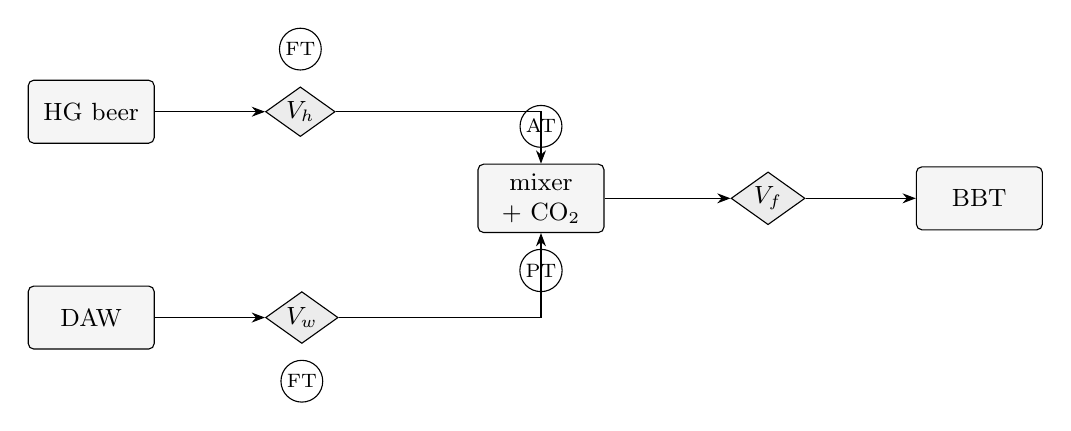
\begin{tikzpicture}[
  font=\small,
  >=Stealth,
  box/.style={draw, rounded corners=2pt, minimum height=8mm, minimum width=16mm, align=center, fill=gray!8},
  valve/.style={draw, shape=diamond, aspect=1.4, inner sep=1pt, fill=gray!15},
  sens/.style={draw, circle, inner sep=1.2pt, font=\scriptsize, fill=white}
]
  \node[box] (bt) {HG beer};
  \node[valve, right=14mm of bt] (vh) {$V_h$};
  \node[sens, above=2mm of vh] (fh) {FT};
  \node[box, below=18mm of bt] (wt) {DAW};
  \node[valve, right=14mm of wt] (vw) {$V_w$};
  \node[sens, below=2mm of vw] (fw) {FT};
  \node[box, right=18mm of vh, yshift=-11mm] (mix) {mixer\\+\ CO$_2$};
  \node[sens, above=2mm of mix] (at) {AT};
  \node[sens, below=2mm of mix] (pt) {PT};
  \node[valve, right=16mm of mix] (vf) {$V_f$};
  \node[box, right=14mm of vf] (bbt) {BBT};
  \draw[->] (bt) -- (vh);
  \draw[->] (vh) -| (mix);
  \draw[->] (wt) -- (vw);
  \draw[->] (vw) -| (mix);
  \draw[->] (mix) -- (vf);
  \draw[->] (vf) -- (bbt);
\end{tikzpicture}
\caption{The three-valve high-gravity blend skid. $V_h$, $V_w$ and $V_f$ are the beer, dilution-water and final valves. FT, PT and AT are flow, pressure and quality measurements. Carbon dioxide is injected at the mixer.}
\label{fig:pid}
\end{figure}

The measurements that the problem is allowed to use are the ones a skid of this kind actually has: volumetric or mass flow on both inlets and on the product, pressures at both headers, at the mix node and at the tank, temperature, valve-stem position, and a quality record of original extract, alcohol, carbon dioxide and dissolved oxygen. The quality record on the outlet is delayed by \SI{12}{\second}. The quality record on the mother beer is delayed by \SI{8}{\second}. Header pressure is available immediately and may be biased. The vena-contracta pressures are not measured. They are computed from \eqref{eq:pvc}.

The design point used throughout the thesis is a cold lager blend at \SI{2}{\celsius}. The mother beer is $A_w=\SI{5.40}{\percent}$ by weight, $E_r=\SI{6.10}{\percent}$ by weight, \SI{5.50}{\gram\per\litre} of carbon dioxide and \SI{8}{ppb} of oxygen. Equation~\eqref{eq:balling} gives an original extract of \SI{16.319}{\degree}P. With the density correlation of Chapter~\ref{ch:methods}, the alcohol is \SI{6.923}{\percent} by volume and the density is \SI{1011.9}{\kilogram\per\cubic\metre}. The sales lager is defined as the $w=0.70$ dilution of that mother beer, carbonated to \SI{5.20}{\gram\per\litre}. It falls at \SI{11.613}{\degree}P and \SI{4.833}{\percent} by volume. A light brand, used as the grade-change target, is the $w=0.58$ dilution at \SI{5.00}{\gram\per\litre} of carbon dioxide, \SI{9.687}{\degree}P and \SI{4.000}{\percent} by volume. The product flow is \SI{20}{\cubic\metre\per\hour}, which is \SI{200}{\hecto\litre\per\hour}. Headers are \SI{4.80}{bar}, \SI{5.30}{bar} and \SI{2.40}{bar} absolute on the beer, the water and the bright tank.

\subsection{Balances}

Let $\dot m_h$ and $\dot m_w$ be the inlet mass flows. The mixer mass $M=\rho V$ obeys
\begin{align}
\label{eq:ode}
M\frac{dA_w}{dt}
&=
\dot m_h(A_{w,h}-A_w) + \dot m_w(A_{w,w}-A_w),
\\
M\frac{dE_r}{dt}
&=
\dot m_h(E_{r,h}-E_r) + \dot m_w(E_{r,w}-E_r).
\end{align}
Water contributes neither alcohol nor extract. Carbon dioxide and oxygen are carried on a volumetric balance because they are measured per litre,
\begin{equation}
\label{eq:co2bal}
V\frac{dc}{dt}
=
Q_h c_h + Q_w c_w + \dot m_{\mathrm{CO_2}} - Q_f c,
\end{equation}
with flows in litres per second and the dose in grams per second. The same form holds for dissolved oxygen, with a dose of zero. The product flow is not an independent input. It is the flow that the final valve passes at the solved mix pressure, and the mass balance $\rho_h Q_h + \rho_w Q_w = \rho_f Q_f$ closes the hydraulics.

At steady state, $w=\dot m_h/(\dot m_h+\dot m_w)$ and \eqref{eq:dilute} holds. The carbon-dioxide dose that hits a target $c^{\star}$ is then fixed by algebra,
\begin{equation}
\label{eq:dosess}
\dot m_{\mathrm{CO_2}}
=
c^{\star}Q_f - c_h Q_h - c_w Q_w.
\end{equation}
For the lager point this dose is about \SI{7.51}{\gram\per\second}, or \SI{27.0}{\kilogram\per\hour}. The number is derived again from the solved flows in Chapter~\ref{ch:estimate}; it is large enough that the injector has to be sized, and small enough that the gas does not change the liquid volume used in the valve equation. The gas is assumed to dissolve when the mix pressure and the vena-contracta pressure both lie above $p_{\mathrm{eq}}$. When they do not, a single-pass disengagement efficiency removes part of the supersaturation. The efficiency is a property of this mixer and this final valve. It is not a universal constant, and at the design point it is inactive because the inequality is satisfied.

\subsection{Why the linear ratio is already outside the tolerance}

Suppose an operator dilutes the mother beer in proportion to original extract, $w = 11.613/16.319 = 0.7116$, on the assumption that original extract itself dilutes. The true blend at that mass fraction has
\[
A_w = 3.843,
\qquad
E_r = 4.341,
\]
and \eqref{eq:balling} returns $p_{\mathrm{OE}} = \SI{11.80}{\degree}P$. The beer is \SI{0.19}{\degree}P high, against a tolerance of \SI{0.05}{\degree}P. The error is four tolerances, and it is produced by arithmetic, not by a faulty valve. The mass fraction that does hit \SI{11.613}{\degree}P is $w=0.700$, and the alcohol there is \SI{4.833}{\percent} by volume. Any controller that trims a volumetric ratio from a linear gain inherits this offset until an integral on the outlet analysis removes it, one mixer volume later. The predictive controller removes it in the model, before the valve moves.

The same algebra shows when the problem becomes infeasible. Alcohol and extract are both multiplied by the single number $w$. A mother beer that arrives with more residual extract and less alcohol---a fermentation that attenuated less---cannot be blended onto an arbitrary pair $(p_{\mathrm{OE}}^{\star},\mathrm{ABV}^{\star})$. One ratio can hit one of them, or a weighted compromise. It cannot hit both. The case study of Chapter~\ref{ch:estimate} uses a mother beer shifted by $+0.45$ percentage points of real extract and $-0.25$ percentage points of alcohol. The original extract of that mother beer hardly changes. The alcohol at the old ratio falls by about \SI{0.21}{\percent} by volume. Restoring the alcohol raises the original extract by about half a degree Plato. The optimisation problem has to say which miss is cheaper. A single-loop extract controller will not say it. It will spend the ratio on extract.

\subsection{Degrees of freedom and constraints}

The fast manipulated vector is
\begin{equation}
\label{eq:u}
\mathbf{u} = (l_h,\, l_w,\, l_f,\, \dot m_{\mathrm{CO_2}}).
\end{equation}
Four quantities can be set: product flow, the mass fraction $w$, the carbon-dioxide concentration, and the mix pressure. That is a square problem when the mother beer is consistent with the brand. Dissolved oxygen is not in the list. It is fixed by the oxygen already in the two liquids and by any pickup at a flashing valve. Temperature is a disturbance from the cellar, slow relative to a grade change. Header pressures are disturbances, measured, and possibly biased. Calcium and any other water ion are monitored constraints of the kind \citet{palmer2013} describes; if they are violated the phase is held, because no $\mathbf{u}$ repairs them.

The inequalities that define a feasible beer are
\begin{align}
\label{eq:ineq}
&0.18 \le l_h,l_w,l_f \le 0.90,
\\
&0 \le \dot m_{\mathrm{CO_2}} \le \dot m_{\mathrm{CO_2}}^{\max},
\\
&|\Delta l| \le \dot l_{\max}\,\Delta t,
\\
&p_{\mathrm{vc},h},\; p_{\mathrm{vc},w},\; p_{\mathrm{vc},f} \ge p_{\mathrm{eq}} + \delta_p,
\\
&p_m \ge p_{\mathrm{eq}} + \delta_m,
\\
&c_{\mathrm{DO}} \le c_{\mathrm{DO}}^{\max}
\quad\text{(alarm if violated; not a manipulated repair)}.
\end{align}
The rate limit $\dot l_{\max}$ is \SI{0.04}{s^{-1}}, a full stroke in \SI{25}{\second}, which is a realistic positioner on a process valve. The pressure margins $\delta_p$ and $\delta_m$ are design choices of the controller, set in Chapter~\ref{ch:methods} so that the solved lager point keeps almost one bar between $p_m$ and $p_{\mathrm{eq}}$ and about \SI{0.37}{bar} between the final vena contracta and $p_{\mathrm{eq}}$.

The objective the controller minimises is the weighted violation of the brand, plus a penalty on valve travel,
\begin{equation}
\label{eq:stage}
\ell
=
\left(\frac{p_{\mathrm{OE}}-p_{\mathrm{OE}}^{\star}}{0.05}\right)^{2}
+
\left(\frac{\mathrm{ABV}-\mathrm{ABV}^{\star}}{0.03}\right)^{2}
+
\left(\frac{c-c^{\star}}{0.05}\right)^{2}
+
0.35\left(\frac{Q_f-Q_f^{\star}}{0.5}\right)^{2}
+
\ell_{\mathrm{soft}}
+
\ell_{\Delta u}.
\end{equation}
The denominators are the tolerances, so a unit of cost is one tolerance of that channel. The weights on extract and alcohol are therefore equal per tolerance, which is the statement that a legal alcohol error and a specification extract error are the same kind of miss. $\ell_{\mathrm{soft}}$ is large when a pressure margin or the oxygen alarm is violated. $\ell_{\Delta u}$ keeps the valves from chattering. Equation~\eqref{eq:stage} is deliberately not a single economic currency in money. A brewery can replace the tolerance weights by costs of beer returns and of lost throughput. The structure of the problem does not change.

\subsection{What is not known well enough to leave in a ratio station}

The valve equation is only as good as $K_v$. A trim that has eroded, or a sizing calculation that was done for water and left uncorrected for beer, moves the true gain by several percent. Several percent of the beer-valve gain at the design point is several cubic metres per hour, which is several tenths of a degree Plato during a grade change. A pressure transmitter that reads \SI{0.10}{bar} high, and a model that believes it, assigns the wrong drop to the beer valve and then attributes the wrong flow to $K_v$. These are the parameters the twin has to estimate before the predictive controller is entitled to its model.

The line resistance is real and, as \eqref{eq:closs} says, only partly structured. The solubility scale $\kappa_{\zeta}$ is real and is not observable from a hydraulic step test, because a step test that stays inside the margin never flashes. It is observable from a bench equilibrium pressure on one sample of known composition. The density contraction is observable because the Coriolis meter reports density directly. A residual network is available for whatever those parameters leave behind, and it is required to conserve mass.

Stiction on the water valve is a discrete defect on top of this continuous model. It is estimated from the smallest command that produces a flow change, and it is compensated by a lead in the command. It is not absorbed into $K_v$, because a deadband and a wrong gain have different signatures: the gain scales every move, and the deadband swallows the small ones.

\subsection{The two technologies, stated as answers to this problem}

The first technology is three-valve nonlinear model predictive control. At each control sample it minimises the sum of \eqref{eq:stage} along a prediction of \eqref{eq:kv}--\eqref{eq:co2bal}, subject to \eqref{eq:ineq}, and it applies the first block of $\mathbf{u}$. The predictor uses the Balling map, so the linear-ratio offset computed above is zero in the model. The predictor uses $p_{\mathrm{eq}}$ from \eqref{eq:zeta} inside \eqref{eq:pvc}, so a move that would flash carbon dioxide is expensive before it happens. The three lifts are one decision vector, so the final valve is not left to discover, after the fact, that the inlet valves have changed the flow it must pass.

The second technology is the physics-informed pressure digital twin that supplies that predictor. It estimates $K_{v,h}$, $K_{v,w}$, $K_{v,f}$, the beer-header bias, $\kappa_{\zeta}$, the density contraction and the effective loss $C_L$ from a short campaign of valve steps, a bench solubility point and the Coriolis density. It trains a residual network under a mass-balance penalty and deploys the network only if held-out steps improve. It reconstructs the mixer composition from the measured flows so that the predictive controller does not wait out the analyser delay, and it inverts a measured water-valve deadband.

The ratio-and-pressure station defined in Section~\ref{sec:tech1lit} remains the baseline. It is the controller a skid has today, retuned by the same gain rules, with the same Balling feedforward an attentive designer would add. The estimation question of Chapter~\ref{ch:estimate} is whether the two technologies improve on that station by enough to matter at the tolerances the brewers already publish, and whether the improvement survives a mother beer that makes the brand infeasible, a sticky water valve, and dilution water that arrives with too much oxygen.

The scope is the skid. Fermentation policy, foam-protein loss, and the design of the deaeration column are upstream. The bright-tank pressure is a boundary condition. The thesis does not claim a plant trial. It claims a formulated problem, two algorithms, and a numerical estimation of how those algorithms behave on a plant model that is more detailed than the model inside the controller.

\chapter{The Two Technologies}
\label{ch:methods}

This chapter specifies the two technologies named in Section~\ref{sec:problem}. The first is the predictive controller that moves the three valves and the carbon-dioxide injector. The second is the twin that estimates the model inside that controller. Both are written so that a programmer can implement them, and so that the numerical choices of the case study are the same choices the text describes.

\section{Three-valve nonlinear model predictive control}
\label{sec:nmpc}

\subsection{Time scales and the model that is predicted}

The controller runs every $\Delta t_c = \SI{4}{\second}$. Between samples the command is held. Inside a prediction the hydraulics are algebraic and the composition is integrated with a step of \SI{2}{\second}. The justification is the bulk-modulus argument of \eqref{eq:bulk}. Pressure equalises in a small fraction of a second. Composition equalises on
\begin{equation}
\label{eq:tau}
\tau = \frac{V}{Q_f}
=
\frac{0.080}{20/3600}
=
\SI{14.4}{\second}
\end{equation}
at the design flow. A horizon of \SI{12}{\second} therefore sees most of one residence time and does not pretend to see the next brand. The analyser delay is \SI{12}{\second} as well, so a controller that used only the outlet analysis would be aiming at a beer that has already left. The controller instead integrates the measured inlet flows through \eqref{eq:ode} and \eqref{eq:co2bal}, and it uses the outlet analysis as a slow correction when it arrives. The state that enters the prediction is that integrated composition, plus a small allowance for flow-measurement noise.

The mother-beer analysis enters with its own delay of \SI{8}{\second}. During those eight seconds the predictor still uses the previous mother beer. The error is visible and short. It is not hidden inside a valve gain.

\subsection{Hydraulics inside each shooting node}

At a candidate lift $(l_h,l_w,l_f)$ and a candidate dose, the mix pressure $p_m$ is the unknown. Inlet densities are evaluated at the inlet compositions. The product density is evaluated at the current mixer composition. With the equal-percentage law \eqref{eq:eqpct} and the sizing law \eqref{eq:kv} at $F_P=F_R=1$,
\begin{align}
\label{eq:qhw}
Q_h
&=
K_{v,h}\,R^{\,l_h-1}
\sqrt{\frac{p_h + b_h - p_m}{\rho_h/1000}},
\\
Q_w
&=
K_{v,w}\,R^{\,l_w-1}
\sqrt{\frac{p_w - p_m}{\rho_w/1000}},
\end{align}
when the drops are positive, and zero otherwise. The symbol $b_h$ is the header bias the model believes. On the true plant it is zero. In a nominal, uncommissioned model it is whatever the transmitter adds. The product flow demanded by mass is
\begin{equation}
\label{eq:qfmass}
Q_f^{\mathrm{mass}}
=
\frac{\rho_h Q_h + \rho_w Q_w}{\rho_f}.
\end{equation}
The blend line then drops by \eqref{eq:darcy}, using the Haaland friction factor at the velocity $Q_f^{\mathrm{mass}}/A_f$, and the final valve passes
\begin{equation}
\label{eq:qfvalve}
Q_f^{\mathrm{valve}}
=
K_{v,f}\,R^{\,l_f-1}
\sqrt{\frac{p_m - \Delta p_{\mathrm{line}} - p_b}{\rho_f/1000}}.
\end{equation}
The scalar residual $Q_f^{\mathrm{valve}} - Q_f^{\mathrm{mass}}$ changes sign between a mix pressure just above the tank and a mix pressure just below the lower header. A bracketed scalar solve, Brent's method in the case study, returns $p_m$. Vena-contracta pressures follow from \eqref{eq:pvc} with the recovery factors of the three trims. If the bracket fails, the node is assigned a large cost and the solver steps away from it. That is a numerical guard, not a physical operating point. At the lager solution of Chapter~\ref{ch:estimate} the residual is closed and the cost of the steady problem is numerically zero.

Density is the affine map identified for \SI{2}{\celsius} in the window of this skid,
\begin{equation}
\label{eq:rho}
\rho
=
\big(999.94 - 1.62\,A_w + 4.05\,E_r\big)
\big(1 - \gamma A_w E_r\big).
\end{equation}
The contraction $\gamma$ is zero in the nominal model and is estimated by the twin. Equilibrium pressure uses \eqref{eq:zeta} with the scale $\kappa_{\zeta}$. Alcohol uses \eqref{eq:abv}. Original extract uses \eqref{eq:balling}. None of these inversions is iterative beyond the scalar pressure solve, because $A_w$ and $E_r$ are states, not outputs that have to be searched for.

\subsection{Composition prediction and carbon-dioxide loss}

From a solved hydraulic node the composition is stepped by the forward Euler form of \eqref{eq:ode} and \eqref{eq:co2bal}. The eigenvalue of the mixer is $-1/\tau \approx \SI{-0.07}{\per\second}$. A step of \SI{2}{\second} multiplies a composition error by about $0.87$ per step and does not oscillate. Euler is therefore enough. A production code can substitute a single exponential on the linear mixer without touching the optimiser.

Delivered carbon dioxide is not identical to the mixer concentration. If the final vena contracta lies below equilibrium, a fraction of the supersaturation leaves the liquid in one pass,
\begin{equation}
\label{eq:strip}
c_{\mathrm{out}}
=
c - \eta\,\max\!\big(0,\; c - \kappa_{\zeta}\zeta\,p_{\mathrm{vc},f}\big),
\end{equation}
with $\eta = 0.35$ for this skid. The same test, with a coefficient of \SI{30}{ppb\per\bar}, adds dissolved oxygen when the margin is negative. Both expressions are inactive when the inequalities in \eqref{eq:ineq} hold, which they do at the design point and throughout the closed-loop runs of Chapter~\ref{ch:estimate}. They exist so that a controller is charged for a flashing move in the prediction, rather than discovering the flash in the bright tank.

\subsection{The program solved at each sample}

The horizon is two move blocks of three integration steps. The decision vector is eight numbers,
\begin{equation}
\mathbf{z} = (l_h^{(1)}, l_w^{(1)}, l_f^{(1)}, \dot m^{(1)},\;
l_h^{(2)}, l_w^{(2)}, l_f^{(2)}, \dot m^{(2)}).
\end{equation}
Inside a block the command is constant, and it is still limited by $\dot l_{\max}$ relative to the previous stem position, so a block cannot teleport a valve. The cost is the sum of \eqref{eq:stage} over the six steps. Soft pressure penalties are quadratic outside the margin, with a weight of $6$ on each squared bar, which is large next to a unit tolerance cost. Valve travel is penalised as $0.4\,\|\Delta\mathbf{l}\|^{2}/0.01$, so a simultaneous move of $0.1$ lift on one valve costs about $0.4$. That is less than one tolerance of extract and enough to suppress chatter.

Bounds are the lift limits and a dose limit of \SI{15}{\gram\per\second}. The initial guess is the move that was applied at the previous sample, copied into both blocks. A sequential least-squares quadratic program then reduces the cost. In the case study the iteration limit is six, which is short on purpose: the warm start is already near a good move, and a valve controller that thinks for longer than a fraction of its sample has missed the sample. The production transcription of the same shooting problem is the real-time iteration \citep{diehl2005,gros2020} solved by an interior-point code \citep{wachter2006,andersson2019}. The case-study solver is a stand-in that minimises the same function. It is not a claim that six sequential-quadratic iterations are a certified real-time iteration.

Only the first block is applied. The stem command is limited once more by $\dot l_{\max}\Delta t_c = 0.16$ lift per sample. The dose is applied as a flow setpoint to the injector, which is fast relative to the mixer.

\begin{algorithm}[htbp]
\caption{One sample of three-valve nonlinear model predictive control}
\label{alg:nmpc}
\begin{algorithmic}[1]
\Require Mixer state, delayed mother-beer analysis, header pressures, previous command, brand setpoint
\State Build the initial guess by repeating the previous command in both blocks
\State Predict the horizon from $\mathbf{z}$ through the algebraic network and the mixer step
\State Minimise the summed stage cost subject to lift and dose bounds
\State Rate-limit the first block against the previous stem position
\State If a deadband estimate is active, lead the water-valve command by that band in the direction of travel
\State Apply the three lifts and the dose; hold them until the next sample
\end{algorithmic}
\end{algorithm}

The deadband lead in line 5 is supplied by the twin and is zero until a stick has been observed. The predictive controller of the first technology does not invent it.

\subsection{Steady solution and the relative-gain array}

The same cost, with the derivatives removed and the composition replaced by its algebraic blend, is a four-variable steady program. At the lager brand, on the plant model, the solution is
\begin{equation}
\label{eq:usteady}
l_h = 0.704,\quad
l_w = 0.711,\quad
l_f = 0.840,\quad
\dot m_{\mathrm{CO_2}} = \SI{7.507}{\gram\per\second}.
\end{equation}
The flows are \SI{13.962}, \SI{6.055} and \SI{20.000}{\cubic\metre\per\hour}. The velocities are \SI{1.134}, \SI{0.762} and \SI{1.078}{\metre\per\second} in the \SI{66}{\milli\metre}, \SI{53}{\milli\metre} and \SI{81}{\milli\metre} bores. Mix pressure is \SI{2.855}{bar} absolute against an equilibrium pressure of \SI{1.905}{bar}. The final vena contracta is \SI{2.279}{bar}. Original extract, alcohol and carbon dioxide meet the brand to three decimals, and dissolved oxygen is \SI{9.22}{ppb}, which is the flow-weighted inlet oxygen and no more. The steady cost is below $10^{-8}$. This is the point a grade change leaves and, for the light brand, the kind of point it has to reach.

Linearising the map $(l_h,l_w,l_f)\mapsto(Q_h,Q_w,p_m)$ with a step of $0.012$ lift gives
\begin{equation}
\label{eq:G}
G
=
\begin{bmatrix}
48.05 & -3.21 & 7.64 \\
-2.59 & 23.09 & 2.64 \\
2.09 & 0.89 & -2.14
\end{bmatrix},
\end{equation}
with flows in cubic metres per hour and pressure in bar, per unit lift. The relative-gain array \eqref{eq:rga} is
\begin{equation}
\label{eq:RGAnum}
\Lambda
=
\begin{bmatrix}
0.87 & 0.00 & 0.13 \\
0.00 & 0.95 & 0.05 \\
0.13 & 0.05 & 0.82
\end{bmatrix}.
\end{equation}
The diagonal dominates. Bristol's test supports pairing beer lift with beer flow, water lift with water flow, and final lift with mix pressure. It does not say the off-diagonal terms are zero. Thirteen percent of the beer-flow relative gain sits on the final valve, and the beer valve moves the pressure. A well-tuned decentralised station can hold this point. A simultaneous grade change excites the off-diagonal terms while the mixer is still full of the previous beer. That is the regime in which the predictive controller has work to do, and it is the regime of the first case in Chapter~\ref{ch:estimate}.

The sign of $G_{33}$ is the operator's sign: opening the final valve lowers the mix pressure. The pressure loop of the baseline is therefore reverse-acting. The predictive controller never needs that sentence, because the final lift is just a coordinate of $\mathbf{z}$.

\subsection{The ratio station used as the baseline}

The baseline is the controller the relative-gain array recommends, built so that the comparison is against a competent station rather than against an untuned one.

Given the delayed mother beer, the station inverts \eqref{eq:balling} for the mass fraction $w_{\mathrm{OE}}$ that hits the extract target, and it inverts \eqref{eq:abv} with the linear part of \eqref{eq:rho} for the mass fraction $w_{\mathrm{ABV}}$ that hits the alcohol target. The feedforward fraction is $0.55\,w_{\mathrm{OE}}+0.45\,w_{\mathrm{ABV}}$. A slow integral on the delayed outlet extract, gain $0.006$ per second, trims that fraction. Mass flows are split by $w$ at the demanded product flow, converted to volumetric setpoints with the linear density, and tracked by incremental proportional--integral loops. With $\Delta t_c=\SI{4}{\second}$ the increments are
\begin{align}
\label{eq:pi}
\Delta l_h
&=
0.018\,(e_h-e_h^{-}) + 0.0018\,e_h\,\Delta t_c,
\\
\Delta l_w
&=
0.028\,(e_w-e_w^{-}) + 0.0030\,e_w\,\Delta t_c,
\\
\Delta l_f
&=
0.12\,(e_p-e_p^{-}) + 0.022\,e_p\,\Delta t_c.
\end{align}
Here $e_h$ and $e_w$ are setpoint minus measurement in cubic metres per hour, and $e_p$ is measured mix pressure minus a fixed pressure setpoint. The fixed setpoint is $p_{\mathrm{eq}}+\SI{0.90}{bar}$ evaluated at the lager steady state, which is \SI{2.805}{bar} absolute. The integral gains were chosen so that $K_I\,G_{ii}\,\Delta t_c$ lies near $0.3$ on the diagonal of \eqref{eq:G}. For the beer valve, $0.0018\times 48.05\times 4 \approx 0.35$. For the water valve, $0.0030\times 23.09\times 4 \approx 0.28$. For the pressure loop, $0.022\times 2.14\times 4 \approx 0.19$. These are the SIMC-sized gains for an algebraic process \citep{skogestad2003,astrom2006}. They are not detuned to make the predictive controller look better.

Carbon dioxide is feedforward from \eqref{eq:dosess} using the measured flows and the delayed mother-beer carbonation, plus an incremental correction from the delayed outlet analysis. The same rate limit is applied to the three lifts. Anti-windup is the incremental form itself: the state of the controller is the stem position, and the stem position is clipped to the lift bounds.

What this station cannot do is revise the pressure setpoint when the brand or the mother beer changes $p_{\mathrm{eq}}$, trade extract against alcohol at the tolerance weights when both cannot be met, or refuse a move whose predicted vena contracta flashes. Those are the jobs of \eqref{eq:stage} and \eqref{eq:ineq}.

\subsection{Offset, feasibility and what the horizon does not prove}

A predictive controller that re-optimises from a measured state removes a constant disturbance that the model can see. It does not remove a constant error in its own gain. If $K_v$ is wrong, the predicted flow of a given lift is wrong, the optimiser asks for the wrong lift, and the outlet integral of a ratio station may still be the faster way home. That is why the first technology, deployed on the nominal model, is not expected to dominate the baseline. The second technology exists to make the model that the first technology trusts.

Feasibility of the inequalities is not guaranteed for every mother beer. When extract and alcohol are inconsistent, the hard bounds on the lifts remain feasible and the quality targets become a soft compromise through \eqref{eq:stage}. When a header pressure collapses so far that the product flow cannot be passed without entering the vena contracta, the soft pressure penalty outranks the flow penalty and the controller gives up flow. The case study does not include a collapse of that size. The header step in Chapter~\ref{ch:estimate} is \SI{0.45}{bar}, and every controller keeps a positive margin.

A terminal constraint to the steady set, of the kind \citet{mayne2000} use to prove stability, is the correct production addition to Algorithm~\ref{alg:nmpc}. The case study does not implement it. The horizon is short, the rate limit is hard, and the steady program is feasible at both brands. The numerical evidence in Chapter~\ref{ch:estimate} is an estimation of closed-loop error, not a Lyapunov certificate. Saying so keeps the first technology in the class of engineering predictive control reviewed by \citet{qin2003} and \citet{maciejowski2002}, where certificates are added when the model and the constraints have settled.

\subsection{A grade change, computed before the valves move}

The light brand asks for $w=0.58$ rather than $0.70$. Product mass flow at the lager density is about \SI{5.61}{\kilogram\per\second}. The beer mass flow therefore falls from about \SI{3.92}{\kilogram\per\second} to about \SI{3.25}{\kilogram\per\second}, and the water mass flow rises by the same \SI{0.67}{\kilogram\per\second}. In volumetric units the beer setpoint moves from \SI{13.96}{\cubic\metre\per\hour} toward about \SI{11.6}{\cubic\metre\per\hour}, and the water setpoint rises from \SI{6.06}{\cubic\metre\per\hour} toward about \SI{8.4}{\cubic\metre\per\hour}. Divided by the diagonal gains, those are lift changes of a few hundredths on the beer valve and about a tenth on the water valve. At \SI{0.04}{lift\per\second} that water-valve move takes about three seconds. Holding the inlet exactly at the new brand after that move would still leave an extract error near \SI{0.7}{\degree}P one residence time later, because $\mathrm{e}^{-1}$ times the \SI{1.93}{\degree}P step has not yet entered the \SI{0.05}{\degree}P band. A controller that is inside the band in \SI{16}{\second} has therefore used an inlet lighter than the new brand while the vessel empties. Section~\ref{sec:firstsample} records that move on the commissioned model. A controller that is still outside the band two minutes later is limited by its model or by its tuning, not by the pipe. Chapter~\ref{ch:estimate} uses that comparison directly.

The carbon-dioxide setpoint falls from \SI{5.20}{\gram\per\litre} to \SI{5.00}{\gram\per\litre} at the same moment. Because the water fraction rises, the dose does not fall in proportion: more uncarbonated water has to be made up. The predictive controller sees both effects in \eqref{eq:co2bal}. The baseline sees them in \eqref{eq:dosess}, which is algebraically the same at steady state and is blind to the trajectory between.

\subsection{Installed gain at the lager lifts}
\label{sec:installed}

The diagonal of \eqref{eq:G} is not an arbitrary linearisation. It is the derivative of \eqref{eq:kv} at the lifts of Table~\ref{tab:steady}, with the mix pressure free to move. Holding the drop fixed isolates the valve. At beer lift $0.704$, $\Phi=0.314$ and $\ln R=\ln 50=3.912$, so
\begin{equation}
\label{eq:dphi}
\frac{\mathrm{d}\Phi}{\mathrm{d}l}
=
\ln R\cdot\Phi
=
3.912\times 0.314
=
1.228.
\end{equation}
A fixed drop would therefore scale the beer flow by $\ln R$ for a unit of lift,
\begin{equation}
\left.\frac{\partial Q_h}{\partial l_h}\right|_{\Delta p}
=
Q_h\ln R
=
13.96\times 3.912
=
\SI{54.6}{\cubic\metre\per\hour}.
\end{equation}
The network gain in \eqref{eq:G} is $48.05$, about twelve percent smaller. The missing part is the rise in mix pressure that follows an opening of the beer valve. That rise shrinks the drop the valve was using, so the installed gain is below the fixed-drop gain. The same comparison on the water valve, $Q_w\ln R = 6.055\times 3.912 = 23.7$ against the network value $23.09$, is almost flat, because the water valve is the smaller flow and moves $p_m$ less. The final valve has the opposite sign: opening it lowers $p_m$, and the inlet valves then pass more flow, which is the positive $G_{13}=7.64$ and $G_{23}=2.64$.

This is the installed characteristic of \citet{iec60534,fisher2005} written as a number the controller can use. An equal-percentage trim was chosen so that the local gain stays near $\ln R$ times the current flow over the whole stroke. At the lager point that product is about \SI{55}{\cubic\metre\per\hour} per unit lift on the beer valve before the network correction, and the correction is modest. A linear trim of the same $K_v$ would have put most of its gain near the shut end and very little at lift $0.70$, which is exactly where this skid lives. The predictive controller does not assume the gain is constant. It re-solves \eqref{eq:kv} at every node. The linear gain is used to size the baseline in \eqref{eq:pi} and to interpret the relative-gain array, not to predict the brand.

\subsection{Bristol's array from the measured gain}
\label{sec:bristol}

The relative-gain array is $G$ multiplied elementwise by the transpose of $G^{-1}$ \citep{bristol1966}. The point of writing the arithmetic is to show that the pairing in Section~\ref{sec:problem} is a property of these three numbers and not a convention copied from a flow--flow--pressure textbook.

Denote the rows of \eqref{eq:G} by the beer flow, the water flow and the mix pressure. The determinant is dominated by the product of the diagonal, $48.05\times 23.09\times(-2.14)$, which is about $-2370$, and the off-diagonal corrections do not change its sign. The $(1,1)$ entry of $G^{-1}$ is the beer-flow response to a beer-lift move after the other two outputs have been held at zero by the other two inputs. Multiplied back by $G_{11}$ it is $\Lambda_{11}=0.87$. The same construction gives $\Lambda_{22}=0.95$ and $\Lambda_{33}=0.82$. Each diagonal entry is the fraction of the open-loop gain that survives when the other loops are closed perfectly. A value near one means the other loops do not steal the actuator. A value near zero would mean the recommended pairing is the wrong one. A negative value would mean the loops fight.

Thirteen percent of the beer-flow relative gain sits on the final valve, and five percent of the water-flow relative gain sits there too. Those are the terms a grade change excites, because a grade change moves all three lifts in the same few seconds, and perfect closure of the other loops is exactly what has not happened yet. At steady state, after the ratio station has settled, the same thirteen percent is a small trim on the pressure loop. The array therefore explains both observations in Chapter~\ref{ch:estimate}: the ratio station can hold a brand, and it is slow when the brand changes. It does not by itself choose the nonlinear map. Balling's denominator is outside $G$, and no arrangement of these nine gains puts it back.

\subsection{How long the horizon has to be}
\label{sec:horizon}

The mixer time constant at the design flow is $\tau=\SI{14.4}{\second}$. The control sample is $\Delta t_c=\SI{4}{\second}$. The prediction uses two move blocks and three Euler steps of \SI{2}{\second} inside each block, so the horizon is
\begin{equation}
T_H = 2\times 3\times 2 = \SI{12}{\second},
\end{equation}
which is $0.83\,\tau$. A step in the inlet composition has, by \eqref{eq:exactdisc}, reached a fraction $1-\mathrm{e}^{-T_H/\tau}=1-\mathrm{e}^{-0.83}=0.56$ of its final value at the end of the horizon. The controller therefore sees a little more than half of the quality move that a valve decision will eventually produce. It does not see the whole settling tail. The tail is left to the next sample, which is the receding-horizon argument: only the first block is applied, and the remainder of the response is re-predicted when the state has moved.

Lengthening the horizon to $2\tau$, about \SI{29}{\second}, would show $86$ percent of the step and would multiply the number of network solves by about two and a half. On a skid whose disturbance is a brand change that is known at the sample it begins, the extra tail is a smaller extract error at the far nodes, already shrinking by $\mathrm{e}^{-\alpha}$ each step, and the decision that matters is the first block. The case study keeps $T_H=\SI{12}{\second}$ for that reason. A disturbance that arrived as an unmeasured ramp over a minute, for example a slow header decay, would justify the longer horizon. The header step in the second scenario is a step, and \SI{12}{\second} covers its onset.

The two blocks are not two independent valve trajectories. Inside a block the command is held, so the eight-vector $\mathbf{z}$ is
\begin{equation}
\mathbf{z}
=
\big(l_h^{(1)},l_w^{(1)},l_f^{(1)},\dot m_{\mathrm{CO_2}}^{(1)},
l_h^{(2)},l_w^{(2)},l_f^{(2)},\dot m_{\mathrm{CO_2}}^{(2)}\big).
\end{equation}
Six Euler steps then see only two values of each actuator. The rate limit is enforced between the previous applied command and the first block, and again between the first block and the second. With a limit of $0.04$ lift per second, the first block may differ from the applied command by at most $0.04\times 4=0.16$ lift, and the second block may differ from the first by the same amount. In two samples the water valve can travel $0.32$ lift. The grade-change arithmetic of the previous subsection needs only about a tenth of a lift on that valve. The rate limit is not what makes the vessel take \SI{14}{\second}. The volume is.

\subsection{A move that the rate limit does price}
\label{sec:travel}

Travel in Table~\ref{tab:kpi} is the sum of absolute lift increments over the run. On the grade change the ratio station travels $7.09$ and both predictive controllers travel about $1.65$. The difference is not a smoother optimum in the abstract. It is the incremental law \eqref{eq:pi} reacting to a flow error that the mixer has not yet produced. At the sample of the setpoint change the ratio station computes new flow setpoints immediately, the flows are still the lager flows, and the errors $e_h$ and $e_w$ are the full step of about $2.4$ and $2.3$ cubic metres per hour. The proportional increments are $0.018\times 2.4$ and $0.028\times 2.3$, a few hundredths of lift, and the integral keeps adding while the vessel is still exchanging. Each later sample sees a flow error of the opposite sign as the valves overshoot the new ratio, and the stems reverse. The sum of those reversals is the travel of $7$.

The predictive controller applies one block that already points at the new steady lifts, then a second block that is close to the first, and then stops. The stage cost charges $0.4\,\|\Delta l\|^{2}/0.01$ for that one move and charges nothing further once the prediction says the vessel will arrive. The travel of $1.65$ is that move plus the small trims that follow the analyser. It is larger than the one-tenth lift of the steady-state arithmetic because the final valve and the dose move as well, and because the first sample cannot jump the whole way when the warm start is the lager command and the iteration budget is six. The budget spends itself on the first sample of the grade change. Later samples start next to a solution and barely move.

The same accounting explains the third scenario, where the commissioned controller travels $0.63$ and the ratio station travels $0.20$. The extra travel is the deadband lead. The stem is commanded across a band of width $0.03$ that produces no flow, so that the flow, when it starts, is the flow the brand asked for. A travel column that is read as ``smaller is always better'' would punish the only controller that has understood the valve. The column is reported so that a reversal hunt, of the kind the untuned absolute-form law produced before the gains of \eqref{eq:pi} were fixed, cannot hide inside a good extract integral.

\subsection{Where the carbon-dioxide dose sits in the same vector}
\label{sec:dosegain}

The dose is the fourth coordinate of each block and it does not appear in $G$, because $G$ was identified on the three lifts with the dose doing whatever holds \SI{5.20}{\gram\per\litre}. Its own gain is algebraic. One gram per second of carbon dioxide, divided by \SI{20}{\cubic\metre\per\hour}, is
\begin{equation}
\frac{1\,\mathrm{g\,s^{-1}}\times 3600}{20\times 10^{3}\,\mathrm{L\,h^{-1}}}
=
\SI{0.180}{\gram\per\litre}
\end{equation}
at the design flow, before the mixer lags it. The stage cost treats \SI{0.05}{\gram\per\litre} as one tolerance, so a dose error of $0.05/0.180=\SI{0.28}{\gram\per\second}$ costs the same, at steady state, as one tolerance of original extract. The optimiser can therefore spend a fraction of a gram per second to protect carbonation without giving up the brand, and it cannot hide a one-gram-per-second mistake. That scaling is why the dose belongs in $\mathbf{z}$ rather than in a slave loop with an unrelated gain. A slave loop can still implement the command. The predictive program decides it, jointly with the lifts, because a water-valve move changes the uncarbonated inlet at the same moment the dose should change.

At the lager point the required dose is \SI{7.507}{\gram\per\second}. The upper bound in \eqref{eq:ineq} is \SI{15}{\gram\per\second}, which is twice the design and is the injector size used in the study. The bound is inactive at both brands. It would become active if the mother beer arrived nearly flat and the product specification stayed at \SI{5.2}{\gram\per\litre}, a case the commissioning range does not include. The program already has the inequality. No new term is required.

The equilibrium pressure moves when the dose moves, because $c$ moves and $p_{\mathrm{eq}}=c/(\kappa_\zeta\zeta)$. A dose increase of \SI{1}{\gram\per\second} raises $c$ by about \SI{0.18}{\gram\per\litre} and $p_{\mathrm{eq}}$ by about $0.18/2.73=\SI{0.066}{bar}$ once the mixer has caught up. The margin constraint sees that rise. A controller that carbonates in a slave loop and only afterwards checks the valve throat will discover the lost margin one analyser delay later. The joint program discovers it inside the shooting node, while the dose is still a decision.

\subsection{The first sample of a grade change}
\label{sec:firstsample}

Table~\ref{tab:horizon} collects the numbers that fix the first sample, so that the horizon is a design choice with units rather than a list of solver options.

\begin{table}[htbp]
\centering
\caption{Prediction budget at the lager flow of \SI{20}{\cubic\metre\per\hour}.}
\label{tab:horizon}
\begin{tabular}{lr}\toprule
Quantity & Value \\\midrule
Mixer volume & \SI{0.080}{\cubic\metre} \\
Residence time $\tau$ & \SI{14.4}{\second} \\
Control sample $\Delta t_c$ & \SI{4}{\second} \\
Euler step inside a block & \SI{2}{\second} \\
Move blocks $\times$ steps & $2\times 3$ \\
Horizon $T_H$ & \SI{12}{\second} \\
Fraction of a step seen, $1-\mathrm{e}^{-T_H/\tau}$ & 0.56 \\
Decision length & 8 \\
Iteration limit & 6 \\
Lift rate limit & \SI{0.04}{lift\per\second} \\
Largest legal first move & 0.16 lift \\
\bottomrule\end{tabular}
\end{table}

At the sample the light brand is requested, the vessel still holds the lager. Original extract is \SI{11.61}{\degree}P against a new target of \SI{9.687}{\degree}P. The error is \SI{1.93}{\degree}P, which is $38.5$ tolerances, and one stage of \eqref{eq:stage} charges about $1.5\times 10^{3}$ on extract alone. Six stages, if the command were left at the lager lifts, charge about $10^{4}$. The horizon sees only $56$ percent of a residence-time step, so a move that merely places the inlet on the new brand produces a predicted extract error that is still enormous at the last node. The solver spends the rate budget to make the inlet lighter than the brand, because that is the only way the predicted error inside \SI{12}{\second} falls by a useful fraction.

On the commissioned model the plant is stepped and then the controller runs, so the new command appears one second later. The lager lifts are $0.703$, $0.713$ and $0.835$. The next applied lifts are $0.543$, $0.873$ and $0.675$. Each coordinate has moved by $0.160$, which is the rate limit of $0.04\times 4$ and not the tenth of a lift that separates the two steady states. Beer flow falls from \SI{13.8}{\cubic\metre\per\hour} to \SI{6.4}{\cubic\metre\per\hour} and water flow rises from \SI{6.1}{\cubic\metre\per\hour} to \SI{10.2}{\cubic\metre\per\hour}. The inlet mass fraction is near $0.39$, not $0.58$. The dose, which had been \SI{7.5}{\gram\per\second}, is raised with the extra water and reaches about \SI{11.6}{\gram\per\second} on the following sample. Four seconds after the upset the extract error is \SI{0.87}{\degree}P. A pure decay at $\tau=\SI{14.4}{\second}$ would still be at $\mathrm{e}^{-4/14.4}\times 1.93=\SI{1.46}{\degree}P$. The difference is the light inlet.

The next samples spend the budget in the other direction. By \SI{16}{\second} the lifts are near $0.66$, $0.81$ and $0.79$, the flows are near \SI{11.4}{\cubic\metre\per\hour} and \SI{8.7}{\cubic\metre\per\hour}, and the extract error is \SI{0.037}{\degree}P, which is the first sample of the strict band in Table~\ref{tab:kpi}. One intermediate sample cuts the product flow to \SI{13.2}{\cubic\metre\per\hour} while the ratio is being restored. That sample is visible in the flow integral. Of the \SI{51}{(\cubic\metre\per\hour)\cdot s} charged to this controller, almost all of it sits in those first \SI{16}{\second}. The extract integral over the whole run is \SI{10.75}{\degree}P$\cdot$s. The same step, decayed at the residence time from an inlet that jumped exactly onto the new brand and integrated to infinity, would cost
\begin{equation}
\int_{0}^{\infty} 1.93\,\mathrm{e}^{-t/14.4}\,\mathrm{d}t
=
1.93\times 14.4
=
27.8
\end{equation}
in degree-Plato seconds. The commissioned run is below that number because the inlet was lighter than the brand, and the flow weight in \eqref{eq:stage} is what the optimiser paid in exchange. The payment is finite. The two other stations on the same run finish at \SI{31.30}{\degree}P$\cdot$s and \SI{32.29}{\degree}P$\cdot$s, and neither enters the band. Their integrals contain the vessel and a model, or a tuning, that keeps feeding the wrong inlet after the vessel could have been emptied.

The nominal predictive controller is the second of those two numbers. It uses the same horizon, the same weights and the same rate limit. The only difference on that run is $\theta$. An extract integral that matches the ratio station, and a tail of about \SI{0.19}{\degree}P, is what an uncommissioned capacity and a \SI{0.10}{bar} header bias produce. The horizon arithmetic does not repair it. The twin does. The six-iteration budget is also visible: the intermediate flow dip is a correction a converged program would have spread more evenly. It does not keep the extract outside the band, and it is one reason the production solver of Section~\ref{sec:rti} replaces the iteration limit by a single warm-started quadratic program.


\section{Physics-informed pressure digital twin}
\label{sec:twin}

\subsection{What the twin contains}

The twin is a second copy of the equations of Section~\ref{sec:nmpc}, with a parameter vector that the skid is allowed to disagree about, a residual correction that is allowed to be zero, and an interface that hands the commissioned copy to Algorithm~\ref{alg:nmpc}. In the classification of \citet{kritzinger2018} it is a twin because that hand-off moves the valves. A display of the same equations would be a shadow.

The parameter vector is
\begin{equation}
\label{eq:theta}
\theta
=
\big(
\log K_{v,h},\;
\log K_{v,w},\;
\log K_{v,f},\;
\log \varepsilon,\;
\log K,\;
b_h,\;
\kappa_{\zeta},\;
\gamma
\big).
\end{equation}
Logarithms keep the capacities, the roughness and the minor-loss coefficient positive. The bias $b_h$ is in bar and may have either sign. The solubility scale and the contraction are estimated from different experiments than the valve steps, because they are barely visible in those steps. They are stored in $\theta$ because the predictor reads them there.

The nominal twin, before commissioning, is the model a project would start from: capacities \SI{29.4}, \SI{13.2} and \SI{58.0}{\cubic\metre\per\hour} against true values \SI{32}, \SI{12} and \SI{64}; roughness \SI{15}{\micro\metre} against \SI{2}{\micro\metre}; minor loss $8$ against $14$; solubility scale $1$ against $0.93$; contraction $0$; and a belief that the beer-header transmitter is truth when it reads \SI{0.10}{bar} high. Those errors are the size of a worn or mis-sized trim and a transmitter that has not been zeroed. They are not a caricature.

\subsection{Commissioning experiment}

Twenty-eight steady points are collected. Each point holds a random lift triple in $[0.40,0.82]$ and a random dose, long enough for the mixer to settle, and records the three flows and the mix pressure. Flow noise is \SI{0.03}{\cubic\metre\per\hour} standard deviation. Pressure noise is \SI{0.008}{bar}. The beer-header measurement used by the estimator is the true header plus \SI{0.10}{bar} plus that noise. Inlet composition is the mother beer of the design point, known because the campaign is run on one tank. This is a few hours of a skid, not a month of history. The point of a physics-based estimator is that a few hours are enough \citep{zheng2023,kadlec2009}.

The hydraulic residual stacks four normalised errors per point,
\begin{equation}
\label{eq:resid}
r
=
\begin{bmatrix}
(Q_h-\tilde Q_h)/0.08 \\
(Q_w-\tilde Q_w)/0.05 \\
(Q_f-\tilde Q_f)/0.08 \\
(p_m-\tilde p_m)/0.02
\end{bmatrix},
\end{equation}
and $\theta$ enters $Q$ and $p_m$ through the network of Section~\ref{sec:nmpc}. The estimator minimises $\|r(\theta)\|^{2}$ by a bound-aware nonlinear least-squares method, starting from the nominal capacities. An approximate covariance follows from the Jacobian $J$ of the converged residual,
\begin{equation}
\label{eq:cov}
\mathrm{Cov}(\hat\theta)
\approx
\hat\sigma^{2}\,(J^{\mathsf T}J)^{-1},
\qquad
\hat\sigma^{2}
=
\frac{\|r\|^{2}}{N-n_{\theta}}.
\end{equation}
Standard errors on $K_v$ are the standard errors on $\log K_v$, multiplied by $K_v$. This is the local Gaussian approximation used throughout nonlinear least squares. It is honest about precision only when the parameters are locally identifiable. Chapter~\ref{ch:estimate} shows that for roughness and minor loss they are not, and the enormous standard errors are the estimator saying so.

\subsection{Parameters that need their own experiment}

Solubility is estimated from one bench point. A sample of known $A_w$, $E_r$ and dissolved carbon dioxide is brought to equilibrium at \SI{2}{\celsius}, the headspace pressure is read, and
\begin{equation}
\label{eq:kappahat}
\hat\kappa_{\zeta}
=
\frac{c}{\zeta_{\mathrm{poly}}(T,E,\mathrm{ABV})\,p_{\mathrm{meas}}}.
\end{equation}
One point identifies one scale. It does not re-identify the polynomial. A brewery that changes beer style enough to leave the polynomial's range repeats the bench point on the new style. That is a laboratory sample, not a flashing test on the line.

Contraction is estimated from the Coriolis density. At each steady point,
\begin{equation}
\label{eq:gammahat}
\hat\gamma
=
\mathrm{median}_{i}
\left(
\frac{1 - \tilde\rho_i/\rho_{\mathrm{lin}}(A_{w,i},E_{r,i})}{A_{w,i}E_{r,i}}
\right),
\end{equation}
taken over points where $A_w E_r > 1$ so that the denominator is not a trace of noise. The median rejects a single bad density reading. The linear map $\rho_{\mathrm{lin}}$ is the parenthesis in \eqref{eq:rho}.

Effective line resistance is not a seventh search variable. After $\varepsilon$ and $K$ have been estimated, or have failed to be estimated, it is computed from \eqref{eq:closs} at $\mathrm{Re}=4\times 10^{4}$, which is the blend-line Reynolds number at the design point. The twin may be rebuilt with that single $C_L$ in place of the pair $(\varepsilon,K)$. In the case study the deployed twin keeps the estimated pair because, although each member is nonsense, the sum $C_L$ lands within three percent of the truth. The text reports both facts so that the next skid estimates $C_L$ directly and does not publish a roughness.

\subsection{The residual network and the mass-balance gate}

After the physical parameters are fixed, the flow residual on the training points is a target for a small network. The input is the standardised vector $(l_h,l_w,l_f,A_w,E_r,p_m)$. The network has one hidden layer of eight hyperbolic-tangent units and a linear output of three flow corrections. Twenty-two of the twenty-eight points train it. Six are held out. Training is Adam for 900 steps at learning rate $0.02$, with a weight decay of $2\times 10^{-3}$.

Every fifth step adds a physics penalty. If $q$ is the physically predicted flow plus the network correction, the penalty is the squared mass imbalance
\begin{equation}
\label{eq:masspen}
\big(\rho_h q_h + \rho_w q_w - \rho_f q_f\big)^{2},
\end{equation}
scaled so that it does not drown a residual that is already at the sensor floor. This is the blend-skid form of the collocation penalty of \citet{raissi2019}. The conservation law is algebraic rather than a differential equation, because the quantity being corrected is a steady flow. \citet{cai2021} make the same substitution whenever a fluid constraint is a flux balance rather than a momentum residual.

The gate is the held-out root-mean-square flow error. If the network increases it, the deployed twin uses $\Delta Q = 0$. The architecture stays in the software so that a later campaign, on a valve whose characteristic is not equal-percentage, can open the gate without a rewrite. \citet{wu2023cerd} and \citet{zheng2023} deploy the network because their reactors have a kinetic discrepancy that the parameters do not absorb. This skid, after $K_v$ and $b_h$ are estimated, does not. The gate is how the twin tells those two situations apart.

\begin{algorithm}[htbp]
\caption{Commissioning of the physics-informed pressure twin}
\label{alg:twin}
\begin{algorithmic}[1]
\Require Step-test records, one bench equilibrium pressure, Coriolis densities
\State Estimate $\log K_v$, $\log\varepsilon$, $\log K$ and $b_h$ by least squares on \eqref{eq:resid}
\State Compute standard errors from \eqref{eq:cov}; if a standard error exceeds the estimate, replace that parameter by the identifiable combination $C_L$
\State Estimate $\kappa_{\zeta}$ from \eqref{eq:kappahat} and $\gamma$ from \eqref{eq:gammahat}
\State Train the residual network on all but six step tests, with the penalty \eqref{eq:masspen}
\State If the held-out flow error rises, set the residual to zero
\State Publish $\theta$ and the residual gate to the predictive controller
\end{algorithmic}
\end{algorithm}

\subsection{The fast state, and the deadband}

During a run the slow parameters stay at the commissioned values. The mixer state is integrated from the measured flows and the delayed mother-beer analysis. This observer is a soft sensor in the sense of \citet{kadlec2009}, and it is almost a balance rather than a regression: if the flows and the inlet composition are right, the mixer composition is determined. Noise of a hundredth of a percent by weight is added in the case study to represent the imperfection of that statement. An unscented filter \citep{julier2004} or a moving-horizon estimator \citep{rao2003} is the right replacement when an inlet meter drops out and the outlet analysis has to carry the state alone. With all three Coriolis meters healthy, the balance is the estimator.

Water-valve stiction is detected as a deadband $S$: the stem does not move until the command has led the reported position by $S$. The case-study fault is $S=0.03$ lift, with no slip jump, which is the stick band of \citet{choudhury2005} reduced to one parameter. The inverse used by the twin-backed controller is
\begin{equation}
\label{eq:invstick}
l_{w,\mathrm{cmd}}
=
l_{w,\mathrm{des}} + S\,\mathrm{sign}(l_{w,\mathrm{des}} - l_{w,\mathrm{pos}}),
\end{equation}
applied only when the desired move exceeds a small threshold, so that a valve already at the setpoint is not dithered. \citet{jelali2010} discuss the limit cycle that a naive inverse can excite. The threshold and the rate limit are what keep \eqref{eq:invstick} from becoming a knocker. The predictive controller that does not receive $S$ has no inverse. It sees a flow that refuses small moves and, if its gain is wrong as well, it walks away from the setpoint.

\subsection{How the twin changes the first technology}

Algorithm~\ref{alg:nmpc} does not contain $\theta$. It contains a model. Commissioning replaces that model. Three substitutions are visible in the closed loop of Chapter~\ref{ch:estimate}.

The capacities and the header bias are the substitutions that repair the grade change. An eight-percent error in $K_{v,h}$ is an error of about \SI{1}{\cubic\metre\per\hour} at the lager point, because the valve is not fully open and the equal-percentage gain is steep. The predictive controller converts that flow error into a composition error and then holds it, because the model believes the composition is already right. The ratio station, which integrates measured flow rather than predicted flow, is less sensitive to $K_v$ and more sensitive to the interaction during the move. The numerical comparison falls out of that difference.

The solubility scale and the contraction are the substitutions that keep the pressure constraint and the alcohol conversion honest. At the design point $\kappa_{\zeta}=0.93$ lowers $\zeta$ from the bare polynomial by seven percent and raises $p_{\mathrm{eq}}$ by the same fraction. A controller that ignores the scale guards the wrong pressure. The contraction shifts density by about \SI{4}{\kilogram\per\cubic\metre} on the mother beer and by about \SI{2}{\kilogram\per\cubic\metre} on the lager. Alcohol by volume, through \eqref{eq:abv}, moves in proportion. The shift is smaller than the alcohol tolerance and is still worth removing, because the tolerance budget should be spent on the mother beer, not on the equation of state.

The deadband inverse is the substitution that matters when the water valve sticks. It does not change the steady mathematics of $w$. It changes the first samples after a small flow error appears.

The residual network, in this campaign, is the substitution that is not made. Publishing that fact is a duty of the estimator. A twin that always adds its network, after the network has failed a hold-out test, is a softer sensor with a harder name.

\subsection{Information, interfaces and the safety boundary}

The twin reads flows, pressures, stem positions, temperature and quality through the OPC UA model of the skid \citep{iec62541}. It writes a recommended $(l_h,l_w,l_f,\dot m_{\mathrm{CO_2}})$ at \SI{4}{\second} intervals. The programmable controller remains the only device that energises a solenoid. It enforces the rate limit again, the lift limits again, and a set of interlocks the optimiser is not allowed to relax: a low bright-tank pressure, a high mixer pressure, a loss of the water-deaeration permissive, and a quality hold if dissolved oxygen or a water analysis crosses the alarm. ISA-88 names the brand change as a phase whose running state may be held by those permissives \citep{isa88}. The predictive controller is a step inside the running state. It is not a replacement for the phase logic.

This boundary is the practical content of the warning in \citet{fuller2020} and \citet{goffi2025} that a twin which can move equipment has to be commissioned inside the interlocks, not beside them. The estimation problem is unaffected. The interlocks define a subset of $\mathbf{u}$ that the least-squares model never sees, because the campaign is run with the interlocks healthy. Extrapolating the twin into a tripped skid is not a use this thesis supports.

\subsection{A hand solution of the lager network}
\label{sec:hand}

The optimiser's steady point can be checked with a calculator, and the check is worth writing down because it is the same arithmetic every shooting node repeats. Take the lifts of \eqref{eq:usteady} and the mother-beer density \SI{1011.9}{\kilogram\per\cubic\metre}. The equal-percentage factor at beer lift $0.704$ is
\begin{equation}
\Phi(0.704) = 50^{-0.296} = \mathrm{e}^{-0.296\ln 50} = \mathrm{e}^{-1.158} = 0.314.
\end{equation}
The effective capacity is $32\times 0.314 = 10.05$ cubic metres per hour. The mix pressure solved by the scalar residual is \SI{2.855}{bar}, so the beer-valve drop is $4.80-2.855=\SI{1.945}{bar}$. With specific gravity $1.012$,
\begin{equation}
Q_h = 10.05\sqrt{1.945/1.012} = 10.05\times 1.386 = \SI{13.93}{\cubic\metre\per\hour}.
\end{equation}
The network solution is \SI{13.962}{\cubic\metre\per\hour}. The difference is the difference between this one-pass density and the density the scalar solver uses after the contraction and the blend have been updated. It is two tenths of a percent. The same arithmetic on the water valve, $\Phi(0.711)=0.323$, effective capacity $3.87$, drop $5.30-2.855=\SI{2.445}{bar}$, specific gravity essentially $1$, gives
\begin{equation}
Q_w = 3.87\sqrt{2.445} = \SI{6.05}{\cubic\metre\per\hour},
\end{equation}
against the solved \SI{6.055}{\cubic\metre\per\hour}.

The blend-line velocity at \SI{20}{\cubic\metre\per\hour} in an \SI{81}{\milli\metre} bore is
\begin{equation}
v_f = \frac{20/3600}{\pi(0.0405)^{2}} = \SI{1.078}{\metre\per\second},
\end{equation}
which is the value in Table~\ref{tab:steady}. The Reynolds number with $\rho\approx\SI{1009}{\kilogram\per\cubic\metre}$ and $\mu=\SI{2.2}{\milli\pascal\second}$ is $4.0\times 10^{4}$. Haaland's formula at $\varepsilon=\SI{2}{\micro\metre}$ returns $f=0.0218$. Then
\begin{equation}
f\frac{L}{D} = 0.0218\times\frac{18}{0.081} = 4.85,
\qquad
C_L = 4.85 + 14 = 18.85,
\end{equation}
and the line drop is
\begin{equation}
\Delta p_{\mathrm{line}} = 18.85\times\frac{1009\times 1.078^{2}}{2}\times 10^{-5} = \SI{0.111}{bar}.
\end{equation}
The pressure immediately upstream of the final valve is therefore about \SI{2.74}{bar}. The final-valve drop down to the tank at \SI{2.40}{bar} is about \SI{0.34}{bar}. With $F_L=0.86$,
\begin{equation}
p_{\mathrm{vc},f} = 2.74 - \frac{0.34}{0.86^{2}} = 2.74 - 0.46 = \SI{2.28}{bar},
\end{equation}
which matches the solved vena contracta of \SI{2.279}{bar}. Equilibrium at \SI{5.20}{\gram\per\litre} and $\zeta=\SI{2.730}{\gram\per\litre\per\bar}$ is \SI{1.905}{bar}. The margin at the narrowest point in the final valve is \SI{0.37}{bar}, and the margin at the mix node is \SI{0.95}{bar}. A designer who stops at the mix-node margin and never computes \eqref{eq:pvc} will believe the skid has a bar of room when the valve throat has a third of that.

The carbon-dioxide check was already done in Section~\ref{sec:build} and closes to \SI{7.51}{\gram\per\second}. The hand solution and the program are the same model. The program is used because a grade change evaluates the residual hundreds of times, not because the residual is obscure.

\subsection{The mixer as a discrete linear system}
\label{sec:discrete}

Once the flows are known, each composition channel is a linear filter. Let $\alpha = Q_f\Delta t/V$ with $\Delta t=\SI{2}{\second}$ and $V=\SI{0.08}{\cubic\metre}$ at the design flow, so $\alpha = 2/14.4 = 0.139$. The exact discretisation of a single well-mixed volume is
\begin{equation}
\label{eq:exactdisc}
x_{k+1} = \mathrm{e}^{-\alpha}\,x_k + \big(1-\mathrm{e}^{-\alpha}\big)\,x_{\mathrm{in}},
\end{equation}
and the Euler step used in the shooting code is the first-order form $x_{k+1}=(1-\alpha)x_k+\alpha x_{\mathrm{in}}$. At this $\alpha$ the two gains on the old state are $\mathrm{e}^{-\alpha}=0.870$ and $1-\alpha=0.861$. The relative difference is one percent. Over a six-step horizon the compounded difference in a step response is a few hundredths of the step, which is smaller than the analyser noise on original extract. Euler is kept because its derivative with respect to the flow, which changes $\alpha$, is obvious to the shooting code. A production build can switch to \eqref{eq:exactdisc} without touching the cost.

The four channels $A_w$, $E_r$, $c$ and $c_{\mathrm{DO}}$ share $\alpha$ and do not share $x_{\mathrm{in}}$. Alcohol and extract see a mass-weighted inlet. Carbon dioxide and oxygen see a volume-weighted inlet plus, for carbon dioxide, the dose divided by $Q_f$. The state transition is therefore diagonal. The output map is not. Original extract and alcohol are nonlinear functions of $A_w$, $E_r$ and $\rho$, and $p_{\mathrm{eq}}$ is a nonlinear function of those and of $c$. That is why a linear model predictive controller built on $G$ in \eqref{eq:G} can coordinate the valves and still miss the brand: $G$ does not contain Balling's denominator. The nonlinear shooting exists for the output map, not because the mixer is a difficult dynamic system.

A linear controller is still the right tool for the diagnosis in \eqref{eq:RGAnum}. It is the wrong tool for the setpoint. The numerical size of the mistake was computed in Section~\ref{sec:problem}: a dilution proportional to original extract misses the true original extract by \SI{0.19}{\degree}P. Any linear gain from flow ratio to original extract that was identified at one brand will carry an offset of that order at the next brand. Integral action removes the offset after the analyser delay. The nonlinear map removes it in the prediction.

\subsection{What one tolerance costs, in the units of the stage cost}
\label{sec:weights}

The denominators in \eqref{eq:stage} are the tolerances, so the numerical weight of each channel is a statement about which miss the brewery will trade. It is worth evaluating the cost at a few concrete errors so the weights are not an unexamined vector.

One tolerance of original extract, with every other error zero, costs $1$. One tolerance of alcohol costs $1$. One tolerance of carbon dioxide costs $1$. A flow error of \SI{0.5}{\cubic\metre\per\hour}, which is \SI{2.5}{\percent} of the design flow, costs $0.35$. A valve move of $0.1$ lift from the previous command costs $0.4\,(0.1)^{2}/0.01 = 0.4$. A mix pressure \SI{0.1}{bar} inside the forbidden side of the margin costs $6\times 0.01 = 0.06$, and \SI{0.5}{bar} inside it costs $1.5$. The pressure penalty therefore overtakes a quality tolerance only when the violation is several tenths of a bar. Small numerical noise in $p_m$ does not dominate the brand. A flashing valve does.

Apply the same arithmetic to the infeasible mother beer of Section~\ref{sec:s2}. The extract-only point misses alcohol by \SI{0.207}{\percent} by volume, which is $0.207/0.03 = 6.9$ tolerances and a cost of about $48$. The alcohol-only point misses original extract by \SI{0.493}{\degree}P, which is $9.9$ tolerances and a cost of about $97$. The weighted point misses extract by \SI{0.167}{\degree}P and alcohol by \SI{0.137}{\percent} by volume, a cost of $(3.34)^{2}+(4.57)^{2}\approx 32$. The predictive controller is not applying a hidden preference for extract. It is applying the squares of the published tolerances. A brewery that considers a tenth of a percent of alcohol more serious than a tenth of a degree Plato changes two numbers in \eqref{eq:stage} and recommissions nothing else.

The flow weight is deliberately smaller than a quality tolerance. On this skid a shortfall of one cubic metre per hour is a scheduling inconvenience, and a shortfall of one degree Plato is a beer that cannot be released. If the skid were the filler and the shortfall were a missed production slot of a high-volume brand, the flow weight would rise. The formulation already has a place for that number.

\subsection{One shooting step, in order}
\label{sec:onestep}

A single evaluation of the horizon at the warm start, which is ``hold the lager command'', during the first sample of the light-brand grade change, does the following.

The mother-beer analysis is unchanged. The setpoint has become \SI{9.687}{\degree}P, \SI{4.000}{\percent} by volume, \SI{5.00}{\gram\per\litre} and \SI{20}{\cubic\metre\per\hour}. The mixer state is still the lager composition, because the valves have not moved. Both blocks of $\mathbf{z}$ are \eqref{eq:usteady}. The network solve returns the lager flows. The mixer step moves the state by $\alpha$ toward an inlet that is still the lager blend, so the predicted original extract stays near \SI{11.61}{\degree}P. The stage cost on extract alone is $((11.61-9.69)/0.05)^{2} \approx 1.5\times 10^{3}$ per step, and six steps cost about $10^{4}$. That number is the signal the solver follows. It is large because the beer in the vessel is still the previous brand, which is a fact, and because the command has not yet been asked to change, which is the degree of freedom.

The solver then shortens the beer lift and lengthens the water lift, subject to the rate limit of $0.16$ lift per four-second sample and to the slower rate inside the prediction. The new flows change $x_{\mathrm{in}}$ through \eqref{eq:dilute}. The predicted extract falls on the time constant \eqref{eq:tau}. Carbon dioxide is recomputed with the new water fraction and the new dose; the dose rises slightly because more water has to be carbonated even though the target concentration has fallen. The pressure residual is re-solved at every node so that the final valve opens as the total flow and the mix density change, instead of letting the pressure loop discover the interaction one sample later. The first block of the improved $\mathbf{z}$ is applied. The next sample repeats the procedure from the new mixer state and the new previous command.

Nothing in that sequence requires the outlet analyser. The analyser arrives \SI{12}{\second} later and trims whatever the flow integration got wrong. On the commissioned model that trim is at the level of the sensor noise. On the nominal model the trim cannot remove a bias that the model interprets as a correct steady state, which is the tail of \SI{0.19}{\degree}P in Section~\ref{sec:s1}.

\subsection{The production solver}
\label{sec:rti}

The case-study program is a single-shooting nonlinear program in eight variables with bound constraints and a smooth cost, apart from the hinges in the soft penalties. Those hinges are squared, so the cost is continuously differentiable and the second derivative jumps. A sequential quadratic solver handles that. The iteration limit of six is a real-time budget, not an optimality certificate. Warm-starting from the previous sample is what makes six iterations enough when the brand is not changing, and what makes the first sample of a grade change the expensive one.

The production form replaces those six iterations by one quadratic program per sample, which is the real-time iteration \citep{diehl2005,gros2020}. Linearise the shooting map at the previous solution $(\mathbf{z},\mathbf{x})$, build the quadratic model of \eqref{eq:stage}, solve it, and apply the first block before the next preparation phase has finished. The preparation of the derivatives can overlap the sample. IPOPT is a reliable way to solve the quadratic model and also the full nonlinear program during commissioning, when there is no sample clock \citep{wachter2006}. CasADi is a reliable way to obtain the derivatives of the network residual and of Balling's map without hand-written Jacobians \citep{andersson2019}. The thesis does not depend on either package being present in the case-study script. It depends on the shooting problem being the one those packages would be given.

Two implementation constraints follow. The scalar pressure solve has to be differentiated through, or replaced by a residual that the nonlinear program carries as an equality. Brent's method on a scalar is easy to run and awkward to differentiate. A production code lifts $p_m$ into the decision vector and writes $Q_f^{\mathrm{valve}}-Q_f^{\mathrm{mass}}=0$ as a constraint at each node. The local derivative of that residual with respect to $p_m$ is negative and bounded away from zero whenever both inlet valves have a positive drop, which they do inside the lift bounds of \eqref{eq:ineq}. The constraint qualification is then the ordinary one for a hydraulic network with a free internal pressure. The second constraint is that the rate limit and the interlocks are enforced in the programmable controller even if the quadratic program returns a point on the wrong side of them. Section~\ref{sec:twin} already assigned that duty to the PLC. The solver is not a safety system.

\subsection{Why roughness and minor loss share one column}
\label{sec:confound}

The line drop \eqref{eq:darcy} depends on $\varepsilon$ only through $f(\varepsilon)$ and on $K$ directly. At a fixed Reynolds number the map $(\varepsilon,K)\mapsto C_L$ is the only map the flows can see, because $C_L$ is the only combination that enters $\Delta p_{\mathrm{line}}$. Differentiating Haaland's formula, $f$ is a slowly increasing function of $\varepsilon/D$. A positive step in $\varepsilon$ and a negative step in $K$ can be chosen so that $C_L$ does not change. The two corresponding columns of the residual Jacobian are then scalar multiples of each other, the Gram matrix $J^{\mathsf T}J$ is singular, and the formal standard error \eqref{eq:cov} diverges. That is what Table~\ref{tab:est} records, in the decision to publish $C_L$ and to withhold a roughness.

The multiplicity is not removed by collecting more points at the same Reynolds number. It is weakly removed by collecting points at very different velocities, because $f$ depends on $\mathrm{Re}$ and $K$ does not, so the two parameters are not in a fixed ratio across the campaign. The commissioning lifts do change the flow, but not by the factor of ten that would separate a smooth-pipe friction factor from a minor loss. A campaign designed to identify roughness would include a near-shut final valve and a wide-open one, and would still be limited by the fact that a hygienic bore at these Reynolds numbers sits in a flat part of the Moody chart. The engineering quantity is $C_L$. The thesis estimates that quantity to two and a half percent and treats the split as unidentified.

The capacities do not have this problem. $K_{v,h}$ scales only $Q_h$, and it scales it with the square root of a drop that the header bias also shifts. Varying the beer lift changes the drop and the flow in a combination a pure bias cannot imitate, because a bias shifts every beer-valve point by the same pressure and a capacity scales them. The standard error of \SI{0.08}{\cubic\metre\per\hour} on a capacity of $32$ is the numerical expression of that excitation. Twenty-eight points were more than the rank of the problem required. They were not more than the noise required.

\subsection{The residual network as a function}
\label{sec:netfun}

Let $\xi\in\mathbb{R}^{6}$ be the standardised feature $(l_h,l_w,l_f,A_w,E_r,p_m)$, with the mean and the scale taken from the training points only. The network is
\begin{equation}
\label{eq:net}
h = \tanh(W_1\xi + b_1),
\qquad
\Delta Q = W_2 h + b_2,
\end{equation}
with $W_1\in\mathbb{R}^{8\times 6}$ and $W_2\in\mathbb{R}^{3\times 8}$. The corrected flow is the physical prediction plus $\Delta Q$. The training loss on a batch is the mean square of $\Delta Q$ against the measured residual, plus the weight decay, plus, every fifth step, a multiple of \eqref{eq:masspen}. The mass penalty is a function of $\Delta Q$ and therefore of $W_2$ and, through $h$, of $W_1$. Its gradient is an ordinary back-propagation of a linear form in the three flows. No collocation point in the sense of a space-time residual of a partial differential equation is required \citep{raissi2019}. The conservation law is the one the flow already lives under.

The hold-out is six points drawn as the last six of the campaign, not re-used in the standardisation or the training. Root-mean-square flow error rises from \SI{0.030}{\cubic\metre\per\hour} to \SI{0.037}{\cubic\metre\per\hour} when $\Delta Q$ is added. The rise is the signature of a model whose physical part has already reached the sensor noise. Adding eight hidden units, forty-eight input weights and twenty-four output weights to a residual whose standard deviation is \SI{0.03}{\cubic\metre\per\hour} on twenty-two points is enough capacity to fit the particular noise of those twenty-two points. The gate compares the two errors and publishes the physical prediction. The weights are kept on disk with the campaign so that a later campaign can be scored against the same architecture. They are not written into the controller.

This is the opposite deployment decision from \citet{wu2023cerd} and \citet{zheng2023}, and it is the same rule. They keep the network because the hold-out improves. This skid drops the network because the hold-out does not. A twin that kept the network anyway would be adding \SI{0.007}{\cubic\metre\per\hour} of invented flow, which is a third of a percent at the beer line and a pointless risk next to a capacity estimate that is already inside \SI{0.1}{\cubic\metre\per\hour}.

\subsection{Observer, delay and the information the analyser still carries}
\label{sec:observer}

The fast observer is the discrete mixer \eqref{eq:exactdisc} driven by measured flows. Its only unknown, between analyser updates, is the inlet composition, and that unknown is replaced by the last mother-beer analysis after eight seconds. The outlet analysis is a measurement of the state that existed \SI{12}{\second}, or six integration steps, earlier. A correction that simply overwrites the current state with the delayed analysis assigns today's vessel the beer of one residence time ago, which is the lager during the first moments of the grade change, and pulls the prediction backwards. The correction used here is therefore applied to the innovation of the delayed prediction: the observer stores a short buffer of predicted outlet values, subtracts the analysis when it arrives, and distributes a fraction of that innovation onto the current state. With healthy flow meters the fraction can be small. The case study adds composition noise of about $0.01$ percentage points by weight so that the controller does not receive the plant state as an oracle.

If the beer flow meter failed, this observer would integrate a lie and the outlet analysis would become the primary measurement. That is the situation in which the moving-horizon estimator of \citet{rao2003} earns its window, and in which an unscented filter \citep{julier2004} is a cheaper approximation. The thesis does not simulate a failed meter. It names the estimator that would replace the balance, and it keeps the balance for the campaign that was actually run. \citet{kalman1960} is the linear special case of both, and it is the right filter for the pressure and flow channels, which are already linear in their noise and are used without a window.

Dissolved oxygen is observed on the same analyser and is not controlled. The observer reports it. The phase logic compares it with \SI{30}{ppb}. The predictive controller includes it in $\ell_{\mathrm{soft}}$ so that a move which would add oxygen by flashing is expensive, and so that a move which cannot remove oxygen already present is not invented. Those are different uses of the same measurement. Conflating them is how a ratio station gets talked into chasing a disturbance it has no actuator for.

\subsection{Faults the cost already contains}
\label{sec:faults}

Four faults are inside the formulation rather than on a list of future work.

A biased beer-header transmitter is $b_h$. It is estimated once and subtracted. Leaving it inside the nominal model produces the grade-change offset of Section~\ref{sec:s1}.

A wrong capacity is an element of $\theta$. It is the difference between the two predictive controllers in every scenario. The ratio station is less sensitive to it because the flow loops close on measured flow. The predictive controller is more sensitive to it because the flow it closes on is a prediction. That asymmetry is the reason the twin is not an optional display next to an otherwise finished controller.

An infeasible brand is a positive minimum of \eqref{eq:stage}. The controller returns the minimiser. It does not return a feasibility flag unless the supervisory station computes the same one-dimensional search in $w$ that Section~\ref{sec:s2} used and compares the two pure compromises with the weighted point. That search is cheap and should be part of the phase start, so that an operator sees ``this mother beer cannot hit both numbers'' before the valves move. The case study performs the search offline and confirms that the closed-loop tail matches it.

A sticky water valve is $S$ in \eqref{eq:invstick}. Undetected, it turns a small flow correction into a delayed jump. Detected, it is a known lead on one command. The eight-second detection delay in the third scenario is a stand-in for a test that looks for a command change with no stem change \citep{jelali2010,choudhury2005}. It is not a claim that eight seconds is the best detector.

Faults that are not inside the formulation are a plugged injector, a failed analyser, a bright-tank pressure below $p_{\mathrm{eq}}$, and a dilution water whose calcium or oxygen certificate is already outside the release limit. The first three are interlocks. The fourth is a hold on the phase. The controller is not asked to blend its way around them.


\subsection{What each technology is for}

The first technology is a way to choose $\mathbf{u}$ when the model is believed. It coordinates the three valves, it uses the nonlinear quality map, and it prices a flashing vena contracta in the same sum as a missed extract. The second technology is a way to decide whether the model should be believed, and to correct the particular parameters that a blend skid gets wrong: capacities, a pressure bias, a solubility scale, a density contraction, a line resistance that must be estimated as a sum, and a deadband. A residual network is part of the second technology and is subject to a hold-out gate.

The next chapter builds the numerical skid on which both are estimated, and it reports what the beer does.

\chapter{System Build and Estimation}
\label{ch:estimate}

The technologies of Chapter~\ref{ch:methods} are estimated on a numerical skid that is more detailed than the controller's nominal model and is fully known, so that every estimate can be scored against a truth. This chapter first builds that skid---pipes, valves, sensors, software and the three upsets---and then reports the parameter estimates and the beer that each controller makes.

\section{System build}
\label{sec:build}

\subsection{Pipes, valves and the sizing that sets the design point}

The beer line is a \SI{66}{\milli\metre} bore, the water line a \SI{53}{\milli\metre} bore, and the blend line an \SI{81}{\milli\metre} bore, \SI{18}{\metre} from the mixer to the final valve. Those bores keep the design velocities near \SI{1}{\metre\per\second}, which is fast enough to stay turbulent and slow enough for a hygienic line. The static mixer and the adjacent pipe hold \SI{80}{\litre}. Minor losses are lumped as $K=14$, a plausible sum for a mixer, a handful of bends and two instrument tees \citep{crane2009,paul2004}. Roughness is \SI{2}{\micro\metre}, a polished stainless bore \citep{white2011}. Viscosity is \SI{2.6}{\milli\pascal\second} on the mother beer and \SI{1.67}{\milli\pascal\second} on the cold water; the blend-line Reynolds number at the design point is $4.0\times 10^{4}$, so $F_R$ in \eqref{eq:kv} is unity and the Haaland friction factor is $0.0218$.

Valve capacities were chosen so that the solved lifts of \eqref{eq:usteady} sit near seven tenths for the inlets and at $0.84$ for the final valve, inside the equal-percentage region and off the seat. The sized coefficients are
\begin{equation}
K_{v,h} = 32,\qquad
K_{v,w} = 12,\qquad
K_{v,f} = 64,
\end{equation}
in cubic metres per hour. Recovery factors are $0.90$, $0.93$ and $0.86$. The final valve is the least recovering of the three, which is why its vena contracta, and not the beer valve's, is the binding carbon-dioxide constraint. A project that buys a high-recovery cage for the final valve buys margin. The controller still has to know $F_L$, because \eqref{eq:pvc} is linear in $1/F_L^{2}$.

Headers are fixed boundary conditions of the cellar: \SI{4.80}{bar} absolute on the beer (\SI{3.79}{bar} gauge), \SI{5.30}{bar} absolute on the water, and \SI{2.40}{bar} absolute on the bright tank (\SI{1.39}{bar} gauge). The tank pressure is the number that makes a non-flashing final valve possible. At \SI{1.90}{bar} of equilibrium pressure, a tank at \SI{2.00}{bar} would put the vena contracta below equilibrium for any useful drop across the final valve. Raising the tank to \SI{2.40}{bar} is a cellar setpoint, decided before the skid is tuned. The predictive controller can trim the mix pressure above that floor. It cannot invent downstream pressure the cellar has not provided.

The carbon-dioxide injector is sized for \SI{15}{\gram\per\second}, twice the lager dose of \SI{7.51}{\gram\per\second}. The dose calculation is the steady balance \eqref{eq:dosess} at the solved flows:
\begin{align*}
c_h Q_h &= 5.50 \times 13.962 \times 1000 = \SI{76791}{\gram\per\hour},\\
c_w Q_w &= 0.03 \times 6.055 \times 1000 = \SI{182}{\gram\per\hour},\\
c^{\star} Q_f &= 5.20 \times 20.000 \times 1000 = \SI{104000}{\gram\per\hour}.
\end{align*}
The difference is \SI{27027}{\gram\per\hour}, or \SI{7.508}{\gram\per\second}, which matches the optimised dose to the last reported digit. The injector is a fourth manipulated variable. It is not one of the three liquid valves. Treating it as a separate flow controller, fed by \eqref{eq:dosess}, is what the baseline does. Putting it inside $\mathbf{z}$ is what the predictive controller does. Both are legitimate; they diverge when the flows are still moving and \eqref{eq:dosess} is being evaluated on a transient.

Dilution water at the design point carries \SI{0.03}{\gram\per\litre} of carbon dioxide and \SI{12}{ppb} of oxygen. The oxygen is inside the band \citet{corosysweb} quote for deaerated water and inside the concern \citet{palmer2013} raise about oxygen picked up at packaging. The mother beer carries \SI{8}{ppb}. Nothing in the build puts an oxygen-removal unit on the skid. The alarm threshold used in the soft cost is \SI{30}{ppb} in the product.

\subsection{Sensors, delays and the numbers the estimator may see}

Each inlet and the product have a Coriolis measurement of flow and density \citep{wang2014}. Pressure is measured at both headers, at the mix node and at the tank. Temperature is measured and, in this study, is constant at \SI{2}{\celsius}. Stem position is measured by the positioner. Original extract, alcohol, carbon dioxide and dissolved oxygen are measured at the outlet with a \SI{12}{\second} delay and with noise of \SI{0.008}{\degree}P, \SI{0.008}{\percent} by volume, \SI{0.015}{\gram\per\litre} and \SI{1.5}{ppb}. The mother-beer analysis is delayed by \SI{8}{\second}. The beer-header transmitter reads \SI{0.10}{bar} high until commissioning removes the bias. These are the only observations Algorithms~\ref{alg:nmpc} and~\ref{alg:twin} receive. The true vena-contracta pressure, the true capacities and the true contraction are withheld and used only as the score.

The plant density uses $\gamma = 1.2\times 10^{-4}$. The plant solubility scale is $0.93$. The plant capacities are the sized values above. The controller's nominal model, until the twin is commissioned, uses the wrong capacities, the wrong roughness, no contraction, a unit solubility scale and the biased header. That split is the whole point of having two technologies rather than one.

Table~\ref{tab:clocks} separates the three clocks, because they are easy to collapse into one ``sample time'' and the collapse hides which delay is physical. The plant is integrated every second with the held command. The supervisory station wakes every four seconds, which is the $\Delta t_c$ of \eqref{eq:pi} and of Algorithm~\ref{alg:nmpc}. Inside a prediction the mixer advances in steps of two seconds, three of them in each move block. The outlet analyser contributes a delay of twelve plant steps, and the mother-beer analysis a delay of eight. A grade change that is ``inside the band in sixteen seconds'' has therefore been seen by four control samples and has not yet been seen by the outlet analyser at all. The sixteen seconds are a statement about the mixer state, which the flow integration observes, and not about a reading that arrives one residence time later and trims a bias. On the commissioned model that trim is at the noise level. On the nominal model the analyser cannot remove the \SI{0.19}{\degree}P tail, because the model treats the biased steady state as the right one.

\begin{table}[htbp]
\centering
\caption{Clocks on the numerical skid. The plant step is the integration of the mixer. The control step is when a new command may be published.}
\label{tab:clocks}
\begin{tabular}{lrr}\toprule
Clock & Period & Count in \SI{16}{\second} \\\midrule
Plant integration & \SI{1}{\second} & 16 \\
Control and ratio station & \SI{4}{\second} & 4 \\
Shooting step & \SI{2}{\second} & 8 \\
Prediction horizon & \SI{12}{\second} & --- \\
Outlet analysis delay & \SI{12}{\second} & --- \\
Mother-beer analysis delay & \SI{8}{\second} & --- \\
\bottomrule\end{tabular}
\end{table}

The noise that is added at each plant step is part of the build, not an afterthought of the plots. Flow noise is \SI{0.02}{\cubic\metre\per\hour} on the beer and the product and \SI{0.015}{\cubic\metre\per\hour} on the water. Mix-pressure noise is \SI{0.006}{bar}. The observer that feeds the predictive controller is the mixer state plus \SI{0.01}{percentage points} by weight on alcohol and real extract and \SI{0.02}{\gram\per\litre} on carbon dioxide. Those magnitudes are smaller than a quality tolerance and larger than zero, so a controller cannot win by reading the plant state as an oracle and cannot be blamed for a sensor it was not given. The same seed is used for all three controllers inside one scenario. A difference in Table~\ref{tab:kpi} is a difference of command, not a difference of noise.

\subsection{Software and the phase that runs a brand}

Figure~\ref{fig:arch} is the runtime. The programmable controller owns the interlocks and the valve solenoids. It publishes measurements and accepts a setpoint. The twin and the predictive controller run in a supervisory station on a \SI{4}{\second} clock. OPC UA carries the named values \citep{iec62541}. The brand change is an ISA-88 phase \citep{isa88}: a start command loads $(p_{\mathrm{OE}}^{\star},\mathrm{ABV}^{\star},c^{\star},Q_f^{\star})$, a running state executes Algorithm~\ref{alg:nmpc}, and a hold state freezes the last legal command if oxygen, a water analysis or a pressure interlock trips. The ratio station, when it is the selected controller, occupies the same phase with \eqref{eq:pi} in place of the nonlinear program. Switching controllers does not switch safety logic.

\begin{figure}[htbp]
\centering
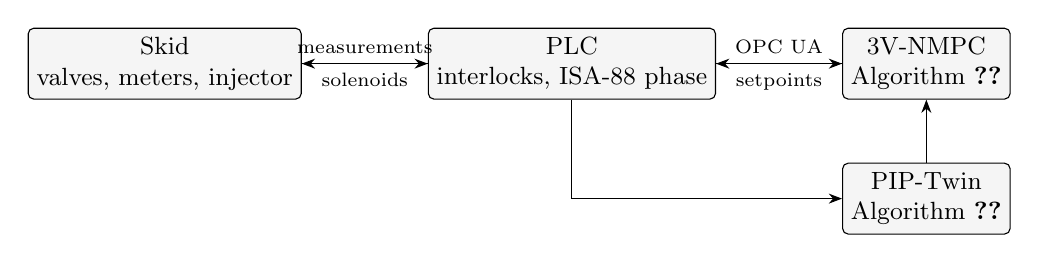
\begin{tikzpicture}[
  font=\small, >=Stealth,
  box/.style={draw, rounded corners=2pt, align=center, minimum height=9mm, fill=gray!8, inner sep=3pt}
]
  \node[box] (skid) {Skid\\valves, meters, injector};
  \node[box, right=16mm of skid] (plc) {PLC\\interlocks, ISA-88 phase};
  \node[box, right=16mm of plc] (nmpc) {3V-NMPC\\Algorithm~\ref{alg:nmpc}};
  \node[box, below=8mm of nmpc] (twin) {PIP-Twin\\Algorithm~\ref{alg:twin}};
  \draw[->] (skid) -- node[above, font=\scriptsize] {measurements} (plc);
  \draw[->] (plc) -- node[above, font=\scriptsize] {OPC UA} (nmpc);
  \draw[->] (nmpc) -- node[below, font=\scriptsize] {setpoints} (plc);
  \draw[->] (plc) -- node[below, font=\scriptsize] {solenoids} (skid);
  \draw[->] (twin) -- (nmpc);
  \draw[->] (plc.south) |- (twin.west);
\end{tikzpicture}
\caption{Runtime of the two technologies. The programmable controller is the only writer of solenoid outputs. The twin publishes a model; the predictive controller publishes a setpoint.}
\label{fig:arch}
\end{figure}

The numerical campaign is the program \texttt{src/simulate\_blender.py}. Commissioning uses a fixed random seed of $29$. Each closed-loop scenario reseeds the sensor noise so that the three controllers see the same noise. The plant, the nominal model and the commissioned twin are the classes defined by the equations of Chapter~\ref{ch:methods}. No gain, weight or capacity reported in this thesis was typed in after looking at a finished plot in order to reverse an inconvenient result. Gains that made the baseline oscillate at the rate limit were reduced, once, to the loop-gain rule of \eqref{eq:pi}, and the scenario was rerun. The tables in this chapter are that rerun.

\subsection{The three upsets}

All three scenarios start at the lager steady point \eqref{eq:usteady} and apply the upset at $t=\SI{20}{\second}$. Integral absolute error is accumulated from the upset to the end of the run. Settling time is the time after the upset at which the original-extract error enters and remains inside \SI{0.05}{\degree}P. If that never happens, the table records a time near the length of the run.

The first upset is a grade change to the light brand: original extract \SI{9.687}{\degree}P, alcohol \SI{4.000}{\percent} by volume, carbon dioxide \SI{5.00}{\gram\per\litre}, flow unchanged. The run lasts \SI{150}{\second}. This is the feasible move. Both extract and alcohol are the $w=0.58$ image of the same mother beer, so a correct model has a solution of zero quality cost.

The second upset keeps the lager brand and changes the supply. Beer-header pressure falls by \SI{0.45}{bar}. Real extract of the mother beer rises by $0.45$ percentage points and alcohol by weight falls by $0.25$ percentage points, with carbon dioxide falling from \SI{5.50}{\gram\per\litre} to \SI{5.15}{\gram\per\litre}. The run lasts \SI{160}{\second}. Section~\ref{sec:s2} shows that this mother beer cannot hit the lager extract and the lager alcohol together. The upset is a test of the compromise, not of tracking.

The third upset keeps the lager brand, raises the dilution-water oxygen from \SI{12}{ppb} to \SI{85}{ppb}, and applies a deadband of $0.03$ lift to the water valve. The twin-backed controller is told the deadband \SI{8}{\second} after it appears, which is a detection delay of the size discussed by \citet{jelali2010}. The run lasts \SI{140}{\second}. The oxygen half of the upset is a test of what estimation must refuse to control.

\section{Estimation}
\label{sec:estimation}

\subsection{The steady point the estimates are taken about}

Table~\ref{tab:steady} is the lager point on the plant. Every quality figure meets the brand. Dissolved oxygen is the inlet blend. The Reynolds number confirms the turbulent valve law. Figure~\ref{fig:pressure} walks the absolute pressure from the beer header to the bright tank. The equilibrium pressure sits below the entire profile, including the final vena contracta. Figure~\ref{fig:char} compares the inherent equal-percentage curve, scaled to the installed flow at lift $0.85$, with the beer flow that the network actually passes as the beer valve moves and the other two lifts stay at the steady point. The installed curve is flatter. A ratio station that was tuned on the inherent gain is mistuned on the skid. The predictive controller never uses the inherent curve as a gain; it re-solves the network.

% auto-generated case-study numbers

\begin{table}[htbp]\centering
\caption{Steady operating point of the sales-gravity lager on the plant model.}
\label{tab:steady}
\begin{tabular}{lr}\toprule
Quantity & Value \\\midrule
Beer-valve lift & 0.704 \\
Water-valve lift & 0.711 \\
Final-valve lift & 0.840 \\
Carbon-dioxide dose (g/s) & 7.507 \\
Original extract ($^\circ$P) & 11.613 \\
Alcohol (\% v/v) & 4.833 \\
Dissolved CO$_2$ (g/L) & 5.200 \\
Dissolved oxygen (ppb) & 9.22 \\
Beer flow (m$^3$/h) & 13.962 \\
Water flow (m$^3$/h) & 6.055 \\
Product flow (m$^3$/h) & 20.000 \\
Beer velocity (m/s) & 1.134 \\
Water velocity (m/s) & 0.762 \\
Product velocity (m/s) & 1.078 \\
Mix pressure (bar a) & 2.855 \\
CO$_2$ equilibrium pressure (bar a) & 1.905 \\
Pressure margin (bar) & 0.950 \\
Final-valve vena contracta (bar a) & 2.279 \\
Blend-line Reynolds number & 40058 \\
Darcy friction factor & 0.0218 \\
Mother-beer mass fraction & 0.7000 \\
\bottomrule\end{tabular}\end{table}

\begin{table}[htbp]\centering
\caption{Steady gain matrix and relative-gain array at the lager point. Outputs are beer flow (m$^3$/h), water flow (m$^3$/h) and mix pressure (bar). Inputs are the three valve lifts.}
\label{tab:rga}
\begin{tabular}{lccc}\toprule
 & Beer lift & Water lift & Final lift \\\midrule
Beer flow & 48.05 & -3.21 & 7.64 \\
Water flow & -2.59 & 23.09 & 2.64 \\
Mix pressure & 2.09 & 0.89 & -2.14 \\
\midrule
$\Lambda$ beer flow & 0.87 & -0.00 & 0.13 \\
$\Lambda$ water flow & -0.00 & 0.95 & 0.05 \\
$\Lambda$ mix pressure & 0.13 & 0.05 & 0.82 \\
\bottomrule\end{tabular}\end{table}

\begin{table}[htbp]\centering
\caption{Commissioning estimates. Standard errors are from the linearised least-squares covariance.}
\label{tab:est}
\begin{tabular}{lrrr}\toprule
Parameter & True & Estimate & Std. error \\\midrule
$K_{v,h}$ (m$^3$/h) & 32.00 & 32.02 & 0.08 \\
$K_{v,w}$ (m$^3$/h) & 12.00 & 12.00 & 0.01 \\
$K_{v,f}$ (m$^3$/h) & 64.00 & 63.99 & 0.12 \\
Header bias (bar) & 0.100 & 0.098 & 0.006 \\
Effective loss $C_L$ & 18.85 & 18.37 & -- \\
Solubility scale $\kappa_\zeta$ & 0.930 & 0.930 & -- \\
\bottomrule\end{tabular}\end{table}

\begin{table}[htbp]\centering
\caption{Closed-loop estimation of beer quality after each upset. IAE is integrated from the upset to the end of the run. Settling time is the time after the upset until original-extract error remains inside $0.05\,^\circ$P.}
\label{tab:kpi}
\resizebox{\textwidth}{!}{%
\begin{tabular}{llrrrrrr}\toprule
Case & Controller & IAE OE & IAE ABV & IAE CO$_2$ & Settle (s) & Travel & Min. margin \\\midrule
S1 grade change & Ratio-PI & 31.30 & 13.48 & 11.81 & 129 & 7.091 & 0.87 \\
S1 grade change & 3V-NMPC & 32.29 & 13.90 & 8.10 & 129 & 1.612 & 0.78 \\
S1 grade change & 3V-NMPC + PIP-Twin & 10.75 & 4.63 & 2.06 & 16 & 1.675 & 0.95 \\
S2 supply upset & Ratio-PI & 12.38 & 21.44 & 2.83 & 139 & 0.833 & 0.86 \\
S2 supply upset & 3V-NMPC & 39.34 & 9.96 & 5.06 & 139 & 0.454 & 0.91 \\
S2 supply upset & 3V-NMPC + PIP-Twin & 20.04 & 17.80 & 1.27 & 139 & 0.414 & 0.90 \\
S3 oxygen and stiction & Ratio-PI & 3.97 & 1.73 & 1.07 & 107 & 0.203 & 0.86 \\
S3 oxygen and stiction & 3V-NMPC & 19.28 & 8.41 & 6.06 & 116 & 0.349 & 0.96 \\
S3 oxygen and stiction & 3V-NMPC + PIP-Twin & 1.29 & 0.56 & 0.95 & $<$1 & 0.634 & 0.91 \\
\bottomrule\end{tabular}}\end{table}


\begin{figure}[htbp]
\centering
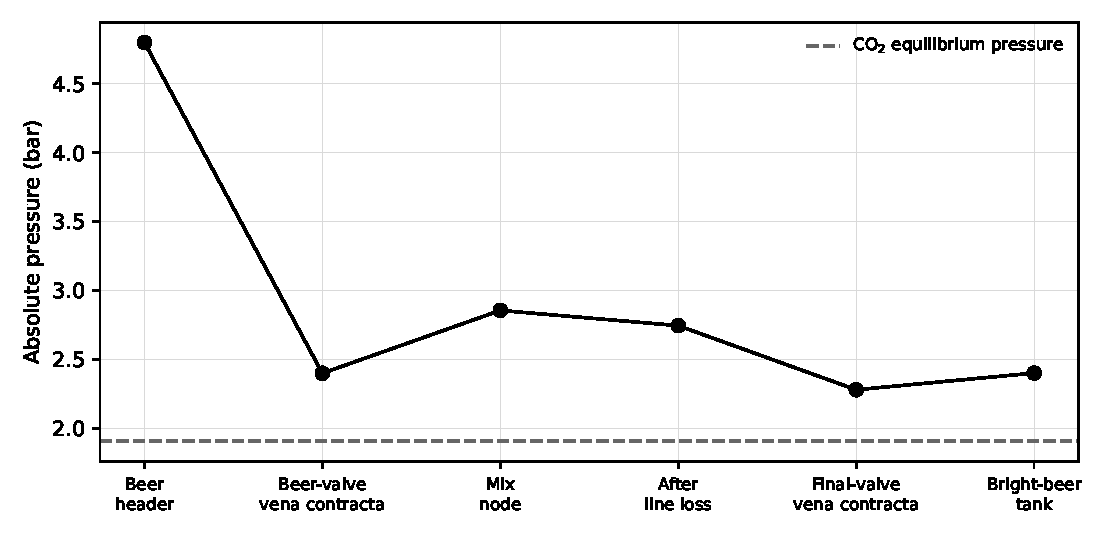
\includegraphics[width=0.92\textwidth]{pressure_profile.pdf}
\caption{Absolute pressure along the beer path at the lager steady point. The dashed line is the carbon-dioxide equilibrium pressure of the finished beer.}
\label{fig:pressure}
\end{figure}

\begin{figure}[htbp]
\centering
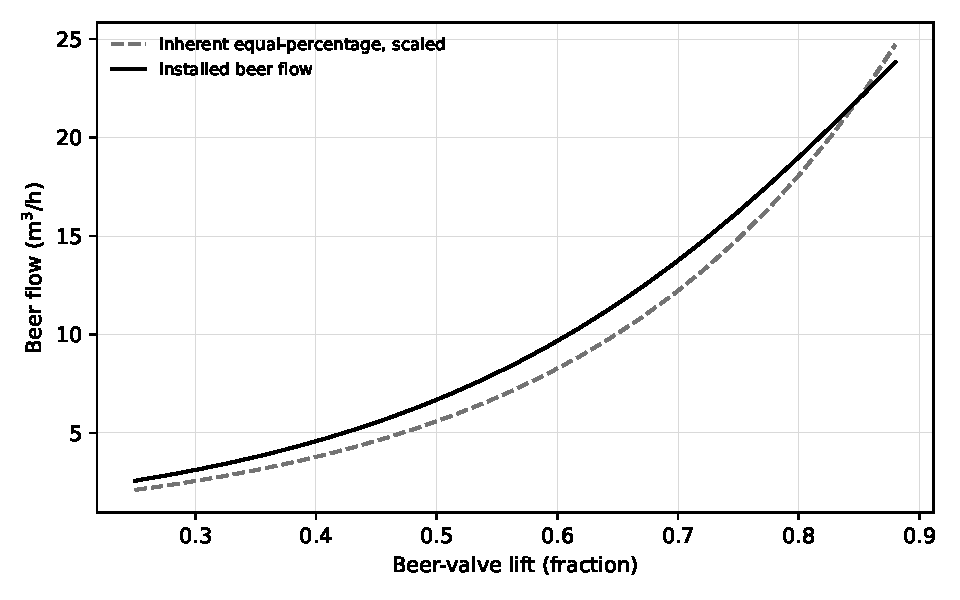
\includegraphics[width=0.78\textwidth]{installed_characteristic.pdf}
\caption{Inherent equal-percentage capacity, scaled to the installed beer flow at lift $0.85$, and the beer flow the network passes with the water and final valves fixed.}
\label{fig:char}
\end{figure}

The gain matrix and the relative-gain array are Table~\ref{tab:rga}, already interpreted in \eqref{eq:G} and \eqref{eq:RGAnum}. The estimation use of that table is practical. Decentralised loops are a fair baseline at this point, so a later improvement has to come from the transient, from the constraint, or from the model, not from a pathological pairing.

\subsection{Commissioning estimates}

Table~\ref{tab:est} is the result of Algorithm~\ref{alg:twin}. The three capacities are recovered to a tenth of a percent, with standard errors of $0.08$, $0.01$ and $0.12$ cubic metres per hour. The header bias is recovered as \SI{0.098}{bar} against \SI{0.100}{bar}, with a standard error of \SI{0.006}{bar}. The solubility scale is \SI{0.930}{} against \SI{0.930}{}. The contraction estimated from \eqref{eq:gammahat} is $1.187\times 10^{-4}$ against $1.20\times 10^{-4}$. These are the parameters the grade change needs, and the campaign of twenty-eight noisy steady points is enough to get them.

Roughness and minor loss are the parameters the campaign cannot separate. The least-squares point drove roughness to several millimetres and the minor-loss coefficient to zero, with a standard error on the minor loss of order $10^{2}$. That point is not reported as a roughness of the pipe, because the standard error says it is not one. The effective resistance $C_L$ computed from the same point at $\mathrm{Re}=4\times 10^{4}$ is $18.37$ against a true value of $18.85$, an error of two and a half percent. The two bad parameters have traded off inside a sum that the pressure drop can see. The next campaign should estimate $C_L$ as a single positive parameter and should stop printing $\varepsilon$.

Figure~\ref{fig:parity} is the beer-flow parity of the nominal model and of the commissioned physical model. The nominal cloud is biased by the wrong capacity and the wrong header. The commissioned cloud lies on the diagonal, inside the \SI{0.03}{\cubic\metre\per\hour} noise that was added to the measurements. The held-out root-mean-square residual of the physical model is \SI{0.030}{\cubic\metre\per\hour}. After the residual network is trained, the same held-out residual is \SI{0.037}{\cubic\metre\per\hour}. The network has learned noise. The gate of Algorithm~\ref{alg:twin} therefore publishes $\Delta Q = 0$, and every closed-loop trace in this chapter that is labelled with the twin is using the calibrated physical parameters only. This is the result anticipated in Section~\ref{sec:twin}. A physics-informed residual is part of the design, and on this skid it is correctly left unused. \citet{kadlec2009} describe the same decision as the maintenance step of a soft sensor: a block that does not improve held-out data is taken out of service.

\begin{figure}[htbp]
\centering
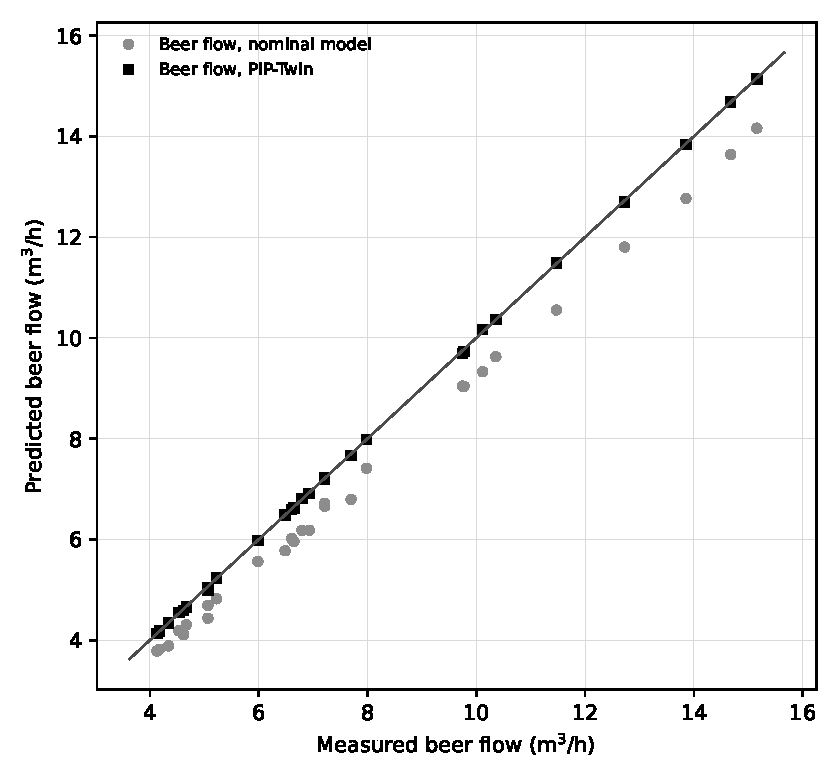
\includegraphics[width=0.72\textwidth]{parity_flow.pdf}
\caption{Beer flow predicted by the nominal model and by the commissioned twin, against the measured beer flow on the commissioning points.}
\label{fig:parity}
\end{figure}

\subsection{Grade change}
\label{sec:s1}

Figure~\ref{fig:s1q} is original extract, alcohol and carbon dioxide through the grade change. Figure~\ref{fig:s1v} is the three lifts. Figure~\ref{fig:bars} collects the extract integrals of all three scenarios. The numbers are the first block of Table~\ref{tab:kpi}.

The ratio station and the predictive controller on the nominal model finish with almost the same extract integral, \SI{31.3}{\degree}P$\cdot$s and \SI{32.3}{\degree}P$\cdot$s. The nominal predictive controller leaves a tail error of \SI{0.19}{\degree}P. Its model, given the wrong capacity and the biased header, believes a lift that is not the lift the plant needs, and re-optimisation from a measured state does not remove an error that the model explains away. The ratio station, integrating measured flow, brings the mean tail error down to \SI{0.02}{\degree}P, but it spends a valve travel of $7.1$ lift-units getting there and its flow integral is \SI{107}{(\cubic\metre\per\hour)\cdot s}, against \SI{51}{} to \SI{68}{} for the predictive controllers. The strict settling test, every sample inside \SI{0.05}{\degree}P for the rest of the run, is not met by either of those two controllers inside the \SI{130}{\second} that remain.

The predictive controller on the commissioned twin meets the strict test at \SI{16}{\second}. The first applied move sits on the rate limit of $0.16$ lift on all three valves: beer flow falls to about \SI{6.4}{\cubic\metre\per\hour} and water flow rises to about \SI{10.2}{\cubic\metre\per\hour}, so the inlet is lighter than the light brand and the extract falls faster than $\mathrm{e}^{-t/\tau}$. Four seconds after the upset the error is \SI{0.87}{\degree}P, against \SI{1.46}{\degree}P for a residence-time decay of the same step. The tail errors, once the flows have returned near \SI{11.5}{\cubic\metre\per\hour} and \SI{8.5}{\cubic\metre\per\hour}, are \SI{0.012}{\degree}P, \SI{0.005}{\percent} by volume and \SI{0.001}{\gram\per\litre}. The extract integral falls from about \SI{32}{\degree}P$\cdot$s to \SI{10.7}{\degree}P$\cdot$s. Carbon dioxide falls from \SI{11.8}{} and \SI{8.1}{} to \SI{2.1}{\gram\per\litre}$\cdot$s. The minimum mix-pressure margin stays at \SI{0.95}{bar}, and no vena contracta crosses equilibrium. Dissolved oxygen stays near \SI{9.7}{ppb}. The maximum extract excursion is \SI{1.92}{\degree}P, which is the size of the setpoint step itself, recorded at the sample the step is applied. Section~\ref{sec:firstsample} gives the lifts.

Table~\ref{tab:s1trace} is that same trajectory at the control samples, taken from the commissioned run. The steady light-brand flows are about \SI{11.6}{\cubic\metre\per\hour} of beer and \SI{8.4}{\cubic\metre\per\hour} of water. The first applied command does not go there. It cuts the beer flow by more than half and raises the water flow above the new steady value, and every lift moves by the legal maximum of $0.16$. The extract error drops from \SI{1.92}{\degree}P to \SI{0.87}{\degree}P in that one sample. The sample at \SI{9}{\second} is the clumsy one: product flow falls to \SI{13.2}{\cubic\metre\per\hour} while the ratio is being put back, and the extract almost stops moving. By \SI{16}{\second} the error is \SI{0.04}{\degree}P and the flows are within about \SI{1}{\cubic\metre\per\hour} of the light-brand steady state. The dose, which is \SI{7.5}{\gram\per\second} on the lager, is above \SI{9}{\gram\per\second} throughout, because the light brand contains more uncarbonated water even after the overshoot has been removed.

\begin{table}[htbp]
\centering
\caption{Commissioned grade change, at the control samples after the upset. Flows are cubic metres per hour and the dose is grams per second.}
\label{tab:s1trace}
\begin{tabular}{rrrrrr}\toprule
Time (s) & $Q_h$ & $Q_w$ & $Q_f$ & Dose & Extract error ($^\circ$P) \\\midrule
0 & 13.8 & 6.1 & 19.9 & 7.7 & $+1.92$ \\
1 & 6.4 & 10.2 & 16.6 & 9.4 & $+1.64$ \\
5 & 9.0 & 10.7 & 19.7 & 11.6 & $+0.68$ \\
9 & 7.7 & 5.6 & 13.2 & 9.3 & $+0.17$ \\
13 & 11.7 & 9.2 & 20.9 & 10.7 & $+0.12$ \\
16 & 11.7 & 9.2 & 20.9 & 10.0 & $+0.04$ \\
21 & 11.6 & 8.4 & 20.0 & 10.1 & $-0.01$ \\
\bottomrule\end{tabular}
\end{table}

The product-flow integral on this path, accumulated in the same way as the extract integral, is \SI{51}{(\cubic\metre\per\hour)\cdot s}. A move that had gone straight to the steady light-brand lifts would have charged much less flow error and left the vessel to forget the lager at $\tau=\SI{14.4}{\second}$. At that rate the error at \SI{16}{\second} would still be about \SI{0.63}{\degree}P, and the strict band would be missed. The \SI{51}{} is the price of not missing it. It is smaller than the ratio station's flow integral of \SI{107}{(\cubic\metre\per\hour)\cdot s}, and it is paid once, at the start, rather than as a reversal hunt across the rest of the run.

The grade-change estimate is therefore not that predictive control beats ratio control. On the nominal model it does not, for extract. The estimate is that predictive control on the commissioned twin brings a feasible brand change inside the extract tolerance in \SI{16}{\second} by spending the rate limit once, and that the same predictive control on the uncommissioned model does not. The first technology needs the second.

\begin{figure}[htbp]
\centering
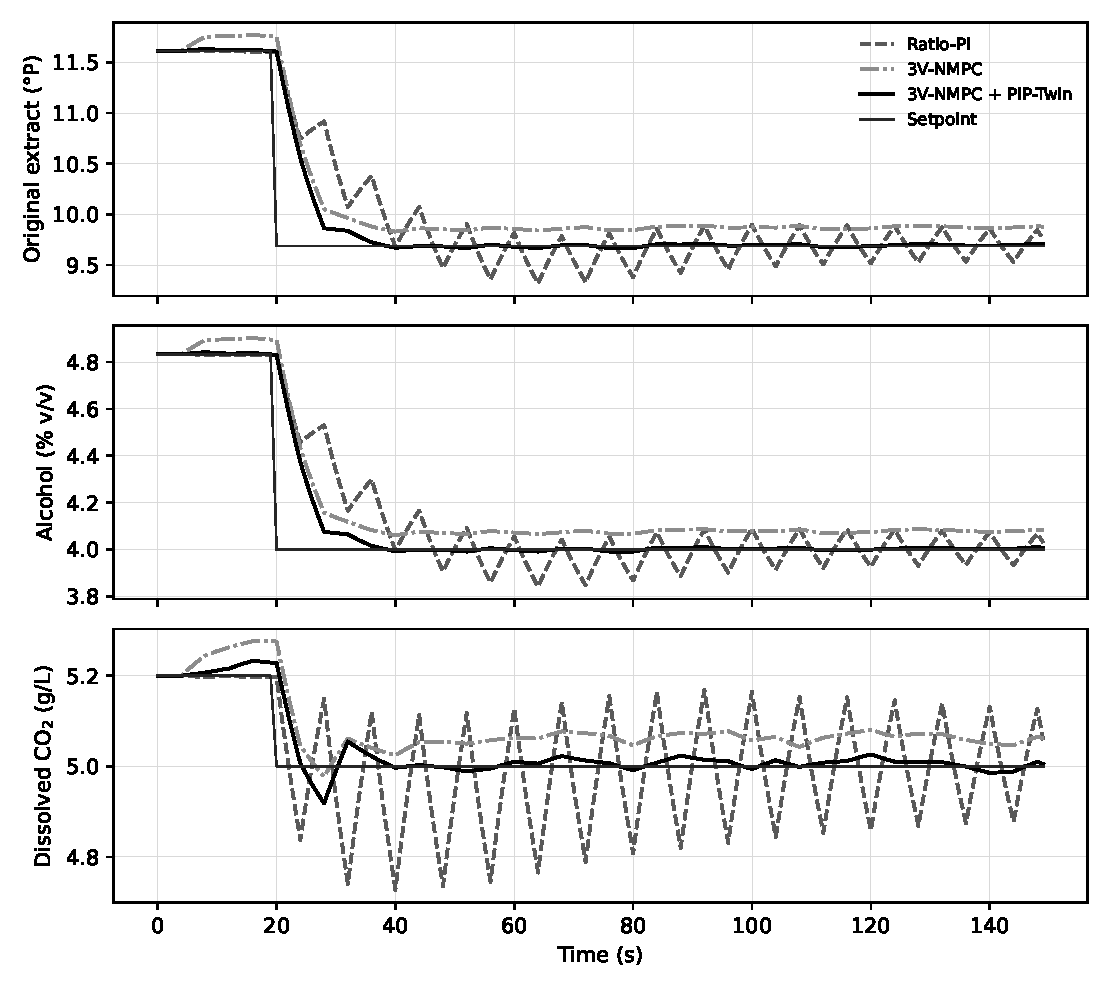
\includegraphics[width=0.92\textwidth]{s1_quality.pdf}
\caption{Grade change from the lager to the light brand at $t=\SI{20}{\second}$. The thin line is the setpoint.}
\label{fig:s1q}
\end{figure}

\begin{figure}[htbp]
\centering
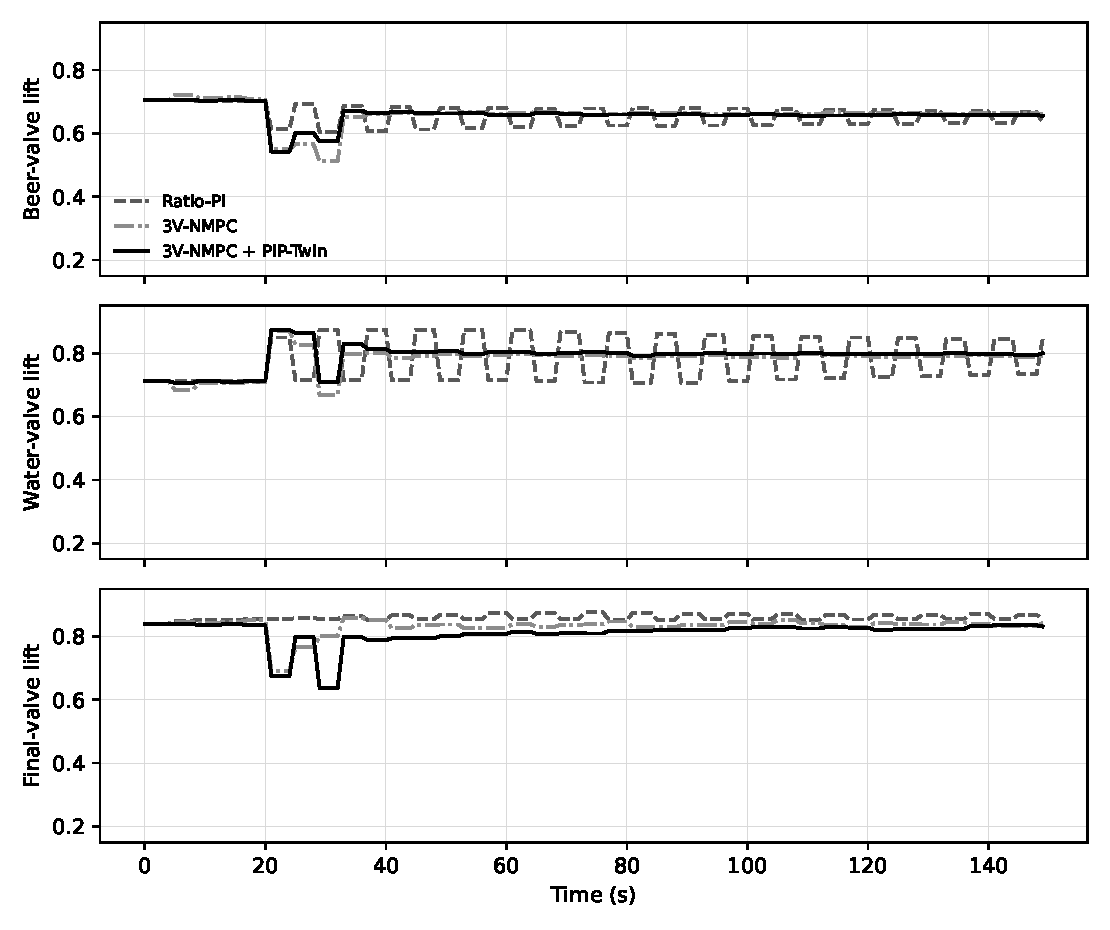
\includegraphics[width=0.92\textwidth]{s1_valves.pdf}
\caption{Valve lifts during the grade change. The ratio station continues to move after the predictive controllers have stopped.}
\label{fig:s1v}
\end{figure}

\begin{figure}[htbp]
\centering
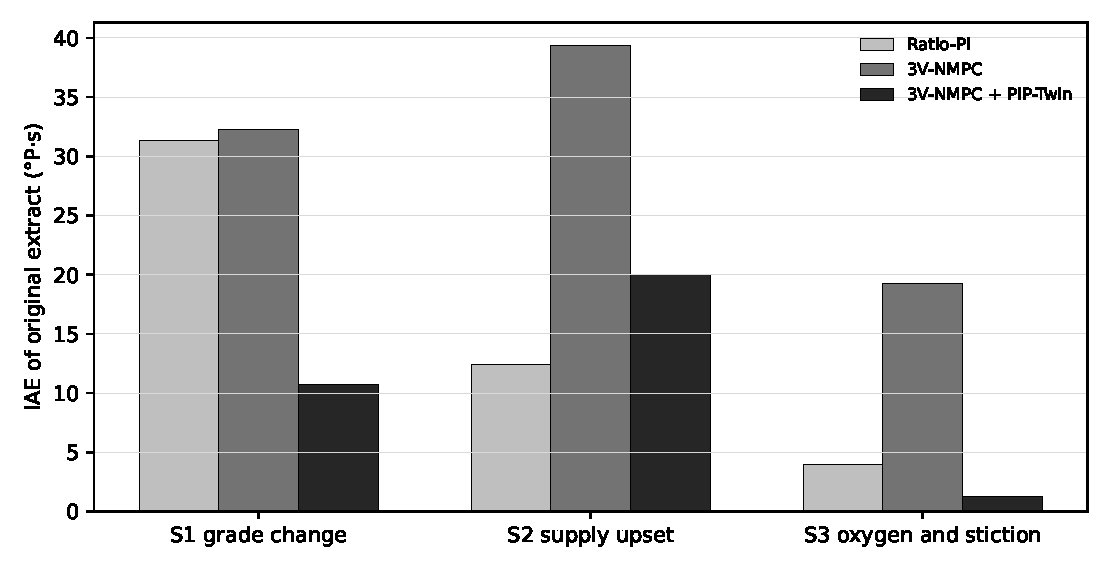
\includegraphics[width=0.92\textwidth]{iae_bars.pdf}
\caption{Integral absolute error of original extract from the upset to the end of each run.}
\label{fig:bars}
\end{figure}

\subsection{A mother beer that makes the brand infeasible}
\label{sec:s2}

After the supply upset the mother beer is $A_w=\SI{5.15}{\percent}$ and $E_r=\SI{6.55}{\percent}$. Its original extract, by \eqref{eq:balling}, is \SI{16.297}{\degree}P, almost unchanged. Its alcohol is \SI{6.617}{\percent} by volume rather than \SI{6.923}{\percent}. A one-dimensional search in $w$ on the plant density gives the two pure compromises and the weighted one. The mass fraction that restores the lager extract is $w=0.702$, and the alcohol there is \SI{4.626}{\percent} by volume, short by \SI{0.207}{\percent}. The mass fraction that restores the lager alcohol is $w=0.733$, and the original extract there is \SI{12.106}{\degree}P, high by \SI{0.493}{\degree}P. The mass fraction that minimises \eqref{eq:stage} without the flow and pressure terms is $w=0.712$, at \SI{11.780}{\degree}P and \SI{4.696}{\percent} by volume. In tolerance units that point costs about $32$. The extract-only point costs about $48$. The alcohol-only point costs about $97$. The weighted optimum sits closer to the extract target because a half-degree extract miss is more tolerances than a fifth of a percent of alcohol, and it does not sit on the extract target, because giving up all of the alcohol is still expensive.

Figure~\ref{fig:s2q} and the second block of Table~\ref{tab:kpi} are what the three controllers do with that geometry. The ratio station's tail is $+\SI{0.091}{\degree}P$ and $-\SI{0.169}{\percent}$ by volume. Its integral on extract has pulled it toward the extract-only point. The nominal predictive controller's tail is $+\SI{0.303}{\degree}P$ and $-\SI{0.080}{\percent}$ by volume: the biased model has chased alcohol and missed the weighted point. The commissioned predictive controller's tail is $+\SI{0.164}{\degree}P$ and $-\SI{0.138}{\percent}$ by volume, which is \SI{11.777}{\degree}P and \SI{4.695}{\percent} by volume, against the calculated optimum of \SI{11.780}{\degree}P and \SI{4.696}{\percent}. The match is inside the noise of the tail average.

No controller records a settling time inside \SI{0.05}{\degree}P, because the weighted optimum itself lies \SI{0.17}{\degree}P off the setpoint. A settling test written on a single setpoint is the wrong test for an infeasible brand. The right test is the distance to the weighted point, and on that test the commissioned controller has arrived. It also holds carbon dioxide to an integral of \SI{1.27}{\gram\per\litre}$\cdot$s against \SI{2.83}{} and \SI{5.06}{}, and product flow to \SI{10.2}{(\cubic\metre\per\hour)\cdot s} against \SI{30.5}{} and \SI{45.2}{}. The header step of \SI{0.45}{bar} is absorbed without a vena-contracta violation. The minimum margins remain above \SI{0.86}{bar}.

The estimate from this upset is that a calibrated predictive controller states the compromise the tolerances asked for, and that a ratio station with an extract integral states a different compromise without saying so. Neither technology creates a second ratio. The alcohol that the fermentation did not produce is not in the skid.

\begin{figure}[htbp]
\centering
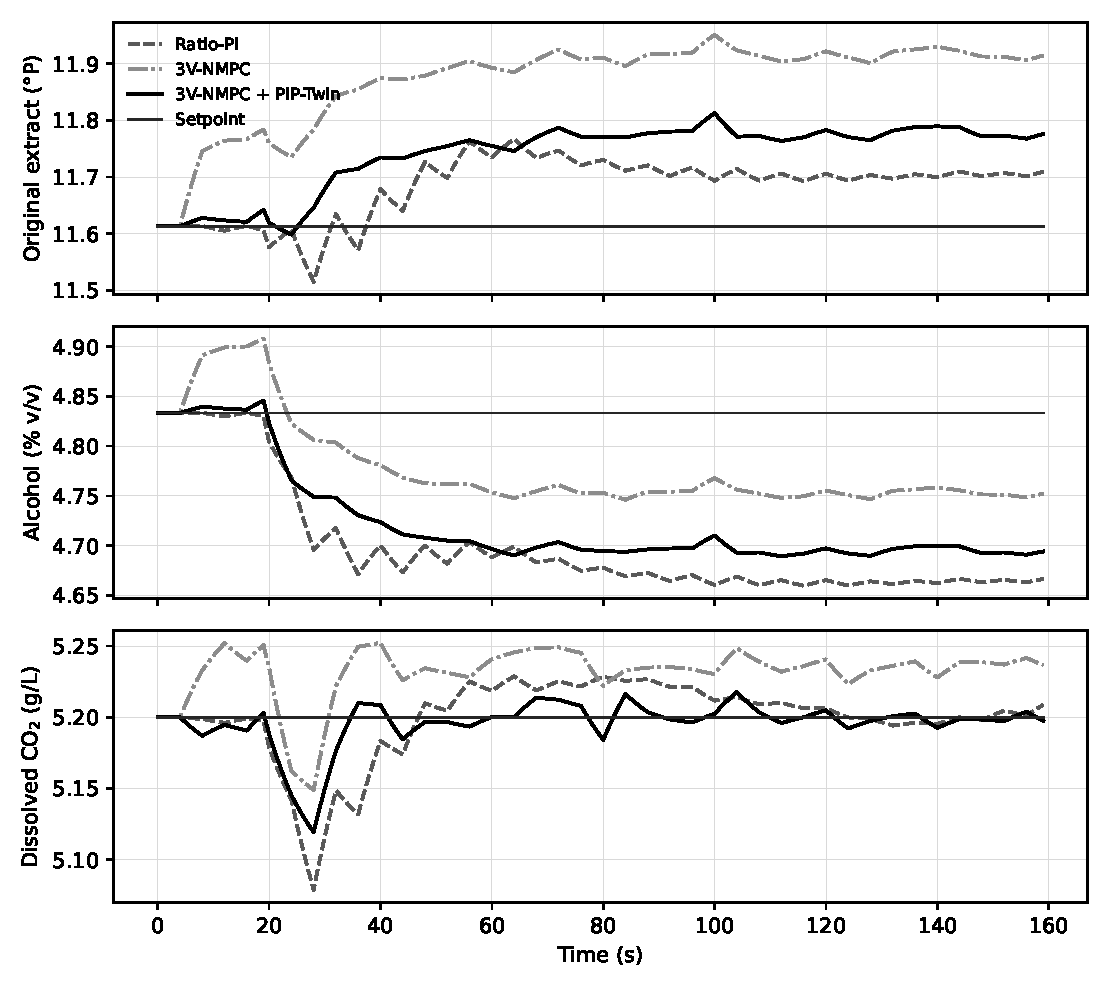
\includegraphics[width=0.92\textwidth]{s2_quality.pdf}
\caption{Supply upset at $t=\SI{20}{\second}$: beer-header pressure down by \SI{0.45}{bar}, mother beer less attenuated. Setpoints are unchanged and are not jointly feasible.}
\label{fig:s2q}
\end{figure}

\subsection{Oxygen and a sticky water valve}
\label{sec:s3}

The oxygen balance at $w=0.70$ with \SI{85}{ppb} in the water and \SI{8}{ppb} in the beer is
\begin{equation}
c_{\mathrm{DO}}
\approx
0.697\times 8 + 0.303\times 85
=
\SI{31.3}{ppb},
\end{equation}
using the volumetric water fraction $6.06/20$. Table~\ref{tab:kpi} reports a maximum dissolved oxygen between \SI{31.2}{ppb} and \SI{31.4}{ppb} for every controller. Figure~\ref{fig:s3q} shows the quality channels; the oxygen itself is the number in the table rather than a fourth trace, because the three traces would overlap. No valve motion removed the oxygen, and no valve motion added a flashing pickup, because the margin stayed above \SI{0.86}{bar}. The alarm at \SI{30}{ppb} is the correct output of the estimator. A controller that moved the water valve to chase a lower oxygen would have left the brand. The phase logic of Section~\ref{sec:build} holds the brand or switches the water source. It does not retune $w$.

The sticky valve is a different estimate. The ratio station's extract integral is \SI{4.0}{\degree}P$\cdot$s and its strict settling time is \SI{107}{\second}, with a tail error of \SI{0.040}{\degree}P. The nominal predictive controller, wrong gain plus an unknown deadband, is worse: an integral of \SI{19.3}{\degree}P$\cdot$s and a tail of \SI{0.144}{\degree}P. The commissioned controller, with the inverse \eqref{eq:invstick} after the eight-second detection delay, keeps the maximum extract error at \SI{0.035}{\degree}P and is therefore inside the settling band from the start of the upset. Its integral is \SI{1.3}{\degree}P$\cdot$s. Valve travel is higher than the ratio station's, $0.63$ against $0.20$, because the inverse takes a deliberate step through the deadband instead of waiting for an integral to creep across it. The beer moves less than the valve does.

The estimate from this upset has two sentences. Dissolved oxygen that arrives in the water is observed and is not a control degree of freedom. Stiction that is estimated and inverted stays inside the extract tolerance; the same predictive controller without that estimate, and with a biased capacity, is the worst of the three stations. Deploying the first technology without the second is not a conservative choice. On this upset it is the expensive one.

\begin{figure}[htbp]
\centering
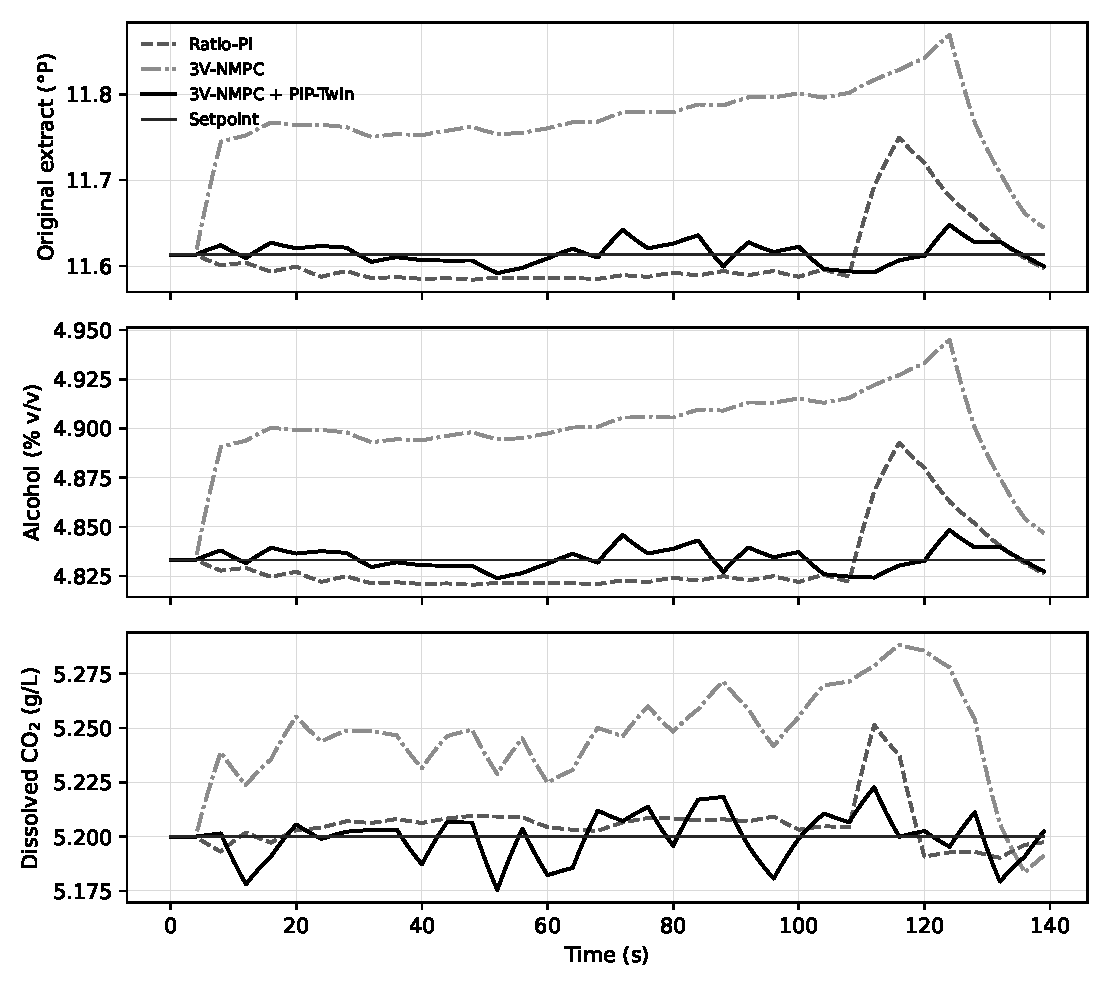
\includegraphics[width=0.92\textwidth]{s3_quality.pdf}
\caption{Dilution-water oxygen raised to \SI{85}{ppb} and a water-valve deadband of $0.03$ lift, from $t=\SI{20}{\second}$. Extract and alcohol stay near the lager setpoint only for the commissioned controller.}
\label{fig:s3q}
\end{figure}

\subsection{Pressure drop, station by station}

The hand solution of Section~\ref{sec:hand} can be read as a commissioning sheet. At the lager point the beer header is \SI{4.80}{bar}. The beer valve consumes \SI{1.945}{bar}. The mix node is \SI{2.855}{bar}. The line, with $C_L=18.85$, consumes about \SI{0.11}{bar}. The final valve consumes about \SI{0.34}{bar} and delivers the beer to a tank at \SI{2.40}{bar}. The throat of that valve is not at \SI{2.40}{bar}. It is at \SI{2.28}{bar}, because $F_L=0.86$ puts the vena contracta \SI{0.46}{bar} below the upstream pressure of the valve and the recovery does not give all of that drop back before the throat. Equilibrium is \SI{1.905}{bar}. The sheet therefore has two margins, \SI{0.95}{bar} at the transmitter and \SI{0.37}{bar} at the throat, and only the second one is the flash margin.

A pressure survey that records the transmitter and not the throat will accept a final valve with a poor recovery factor. The controller cannot see the throat either. It computes it from $F_L$, which is a number from the valve data sheet \citep{fisher2005,iec60534}, and from the pressures it can measure. Commissioning checks the computation by confirming that the measured mix pressure, the measured tank pressure and the measured flow are consistent with the $C_L$ and the $K_{v,f}$ in Table~\ref{tab:est}. They are, to the standard errors in that table. A discrepancy larger than those standard errors is a fouled mixer or a wrong recovery factor, and it is a reason to reopen the gate on the residual network rather than a reason to detune the brand.

The velocities that go with this sheet are \SI{1.134}{\metre\per\second} on the beer, \SI{0.762}{\metre\per\second} on the water and \SI{1.078}{\metre\per\second} on the product. All three are in the turbulent hygienic range. The water line is the slowest, which is one reason a sticky water valve is the fault worth injecting: a valve that spends its life at a modest opening and a modest velocity is the valve whose stem is most likely to sit. The beer valve, at a higher opening and a higher gain, shows a stick as a flow error immediately. The water valve can hide a deadband of $0.03$ lift inside a flow change of less than one cubic metre per hour until the grade change asks it to move.

\subsection{What was estimated, and what a brewery still has to measure}

The parameter estimation is Table~\ref{tab:est}: capacities and header bias to a small fraction of their values, solubility scale and contraction from their own one-point experiments, line resistance as a sum and not as a roughness. The quality estimation is Table~\ref{tab:kpi} together with the weighted point of Section~\ref{sec:s2}. On a feasible grade change the commissioned controller is inside \SI{0.05}{\degree}P in one residence time, and the uncommissioned predictive controller is not better than ratio control. On an infeasible mother beer the commissioned controller sits on the tolerance-weighted compromise to three decimal places of the steady calculation. On a sticky water valve it holds the brand, and on oxygenated dilution water it reports an alarm that every controller's product confirms at \SI{31}{ppb}.

Several limits are part of the estimate rather than footnotes under it. The plant and the twin share the same equation structure. A real trim that is not equal-percentage, or a mixer that is not a single volume, would open the residual-network gate and should be tested by repeating the hold-out on plant step tests before the gate is trusted. The pressure solver and the short sequential-quadratic program are not a certified real-time iteration; the timing result is that a \SI{12}{\second} horizon of this size solves in well under the \SI{4}{\second} sample on a desktop, which is necessary and not sufficient for an embedded controller. The terminal constraint that would support a stability argument was not imposed. Sensor faults were noise and one bias, not a failed meter. The bright-tank pressure was a boundary that had already been raised high enough to make the vena contracta feasible. A cellar that cannot provide that pressure has a different problem, and the controller will correctly spend flow to protect $p_{\mathrm{eq}}$ only inside the limits of the headers it is given.

Foam, yeast stress and the flavour match between a high-gravity beer and a sales-gravity beer remain the fermentation questions reviewed by \citet{stewart2010}, \citet{gibson2007} and \citet{bamforth2009}. The skid does not answer them. What it can answer, and what this estimation measured, is whether the beer that dilution is capable of making is the beer that leaves the final valve. With the three lifts and the carbon-dioxide dose chosen by the predictive controller, and with the model of that controller commissioned by the twin, the feasible brand is inside the extract tolerance sixteen seconds after the change, the infeasible brand leaves at the compromise the tolerances define, and the oxygen that no valve can remove is reported rather than stirred.


\bibliographystyle{unsrtnat}
\bibliography{refs}

\end{document}
